\documentclass[10pt,a4paper]{article}

\usepackage[utf8]{inputenc}
\usepackage[margin=1in]{geometry}
\thispagestyle{empty}

\usepackage{amsmath}
\usepackage{amsfonts}
\usepackage{amssymb}

\usepackage{parskip}

\usepackage{listings}
\usepackage{xcolor}

\usepackage{enumerate}

\usepackage{hyperref}

\usepackage{float}
\restylefloat{figure}
\usepackage[font=small,labelfont=bf]{caption}
\usepackage{wrapfig}

\usepackage{graphicx}
\restylefloat{figure}

\usepackage{cancel}

\usepackage{multicol}
\setlength{\columnsep}{22pt}

\usepackage{colortbl}

\usepackage{cases}

\usepackage{verbatim}

\title{Redes y Comunicaciones de Datos II}
\author{Cristian Escudero \\ \small{Resumen}}

\begin{document}
\maketitle

\section{La Capa de Red}

La \textbf{capa de red} (CdR) se encarga de llevar los paquetes desde el origen hasta el destino, lo que puede requerir muchos saltos por enrutadores intermedios. Contrasta con la \textbf{capa de enlace de datos} (CED), cuya función es la de mover tramas de un extremo del cable al otro. La CdR es la capa más baja que maneja la transmisión de \textbf{extremo a extremo}.

La CdR debe:
\begin{itemize}
\item Conocer la \textbf{topología} de la \textit{subred} de comunicación y elegir las rutas adecuadas a través de ella.
\item Tener cuidado al escoger las rutas para no sobrecargar algunas de las líneas de comunicación y los enrutadores y dejar inactivos a otros.
\item Cuando el \textit{origen} y el \textit{destino} están en redes diferentes, se encarga de solucionar los problemas que surjan.
\end{itemize}

\subsection{Aspectos de diseño de la capa de Red}

\subsubsection{Servicios proporcionados a la capa de Transporte}

Objetivos de los servicios proporcionados por la CdR:
\begin{enumerate}
\item Deben ser independientes de la tecnología del enrutador.
\item La \textbf{capa de transporte} (CdT) debe estar \textbf{aislada} de la cantidad, tipo y topología de los enrutadores presentes.
\item Las direcciones de red disponibles para la CdT deben seguir un plan de numeración uniforme, aun a través de varias LANs y WANs.
\end{enumerate}

\begin{figure}[ht!]
  \caption{Diferencia gráfica entre servicios orientados y no orientados en la CdR.}
  \label{fig:redes_cons_clns}  
  \centerline{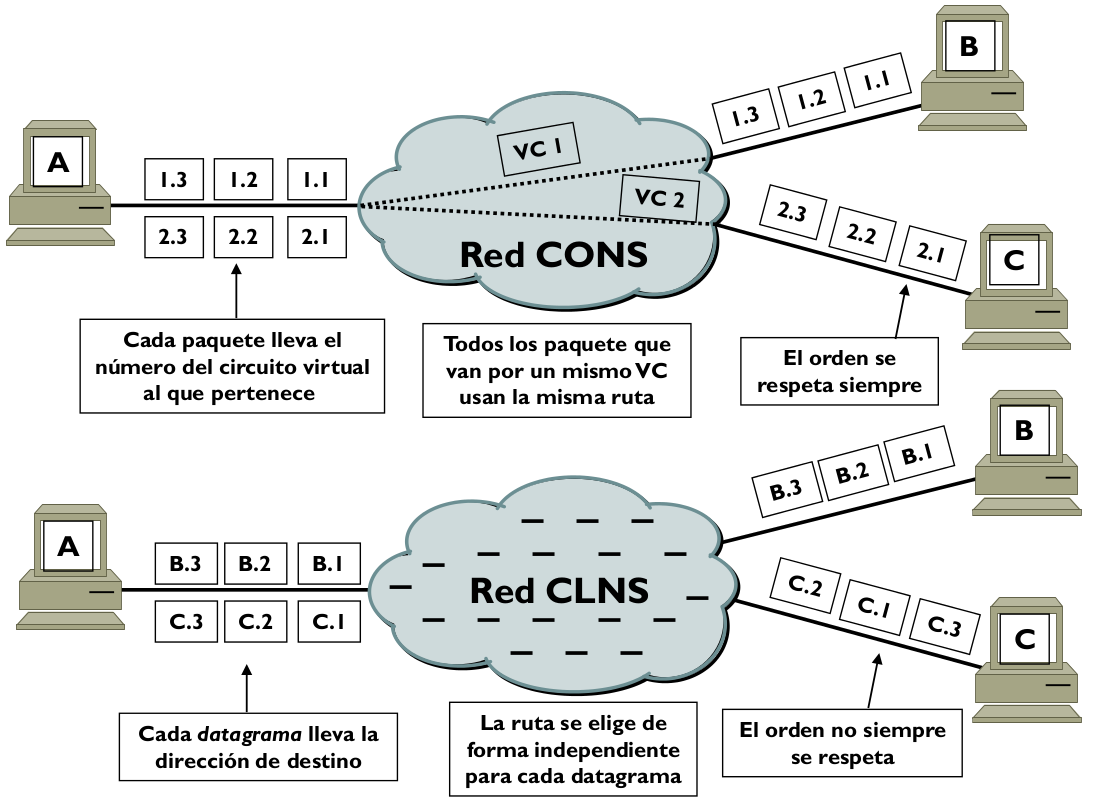
\includegraphics[width=0.8\textwidth-\fboxrule-\fboxrule]{imgs/redes_cons_clns.png}}  
\end{figure}

\subsubsection{Implementación del servicio no orientado a la conexión}

\underline{\textbf{{Servicio no orientado a la conexión:}}}
Los paquetes se colocan individualmente en la subred y se enrutan de manera independiente. No se necesita una configuración avanzada. Los paquetes son referidos como \textbf{datagramas} y la subred se conoce como \textbf{subred de datagramas}. 

\underline{\textbf{{Servicio orientado a la conexión:}}}
Antes de poder enviar cualquier paquete de datos, es necesario establecer una ruta del enrutador de origen al de destino. Esta conexión se conoce como \textbf{circuito virtual} (CV), y la subred se conoce como \textbf{subred de CVs}. 

El algoritmo que maneja las tablas y que realiza las decisiones de enrutamiento se conoce como \textbf{algoritmo de enrutamiento}.

\begin{figure}[ht!]
  \caption{Enrutamiento dentro de una: subred de datagramas (\textit{arriba}), subred de CVs (\textit{abajo}).}  
  \label{fig:orientado_conexion}  
  \hbox{
  \centerline{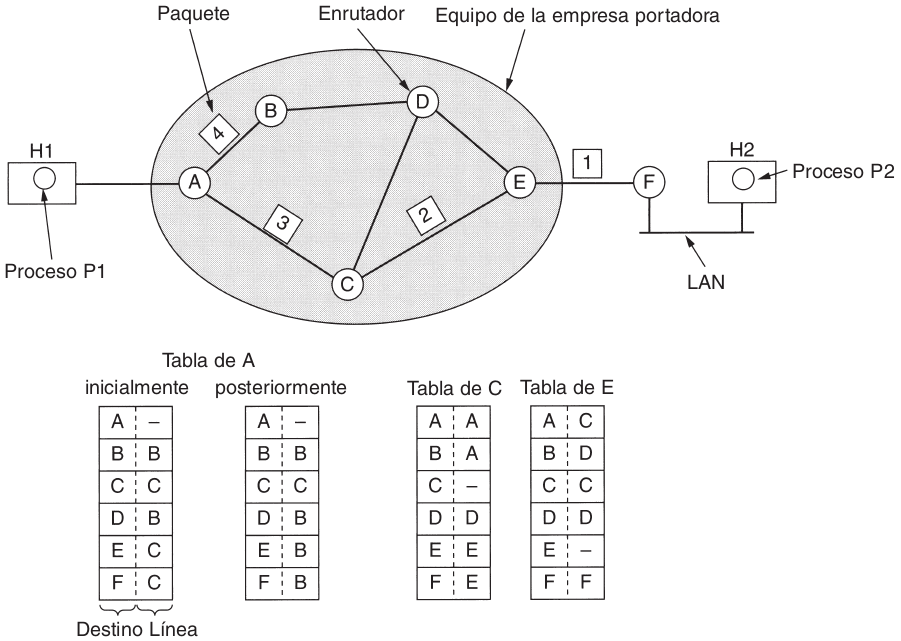
\includegraphics[width=0.9\textwidth-\fboxrule-\fboxrule]{imgs/orientado_conexion.png}}
  }
  \vspace{25pt}
 \hbox {
 \centerline{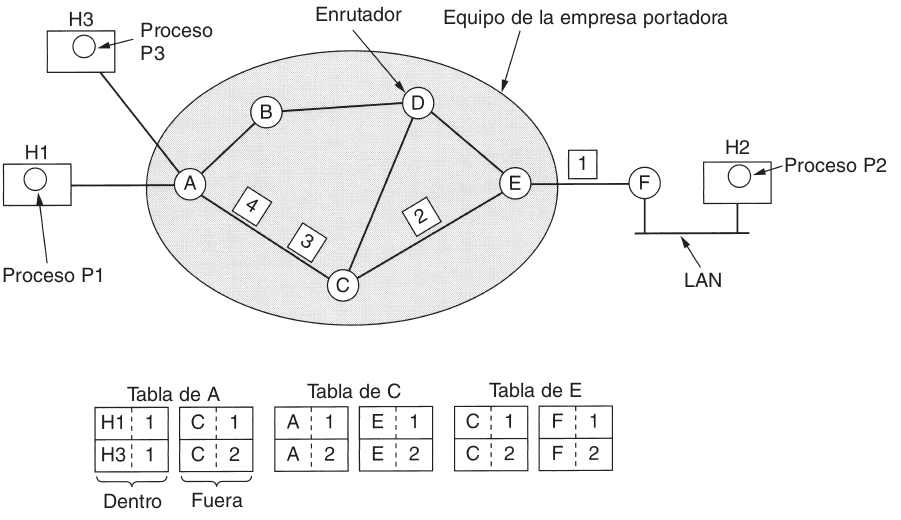
\includegraphics[width=0.9\textwidth-\fboxrule-\fboxrule]{imgs/no_orientado_conexion.png}}}
\end{figure}

\subsubsection{Implementación del servicio orientado a la conexión}

Necesitamos una subred de CVs para evitar la necesidad de elegir una nueva ruta para cada paquete enviado. Cuando se establece una conexión, se elige una ruta de la máquina de origen a la de destino como parte de la configuración de conexión y se almacena en tablas dentro de los enrutadores. Esa ruta se utiliza para todo el tráfico que fluye a través de la conexión. Cuando se libera la conexión, también se termina el CV. Cada paquete lleva un \textbf{identificador} que indica a cuál CV pertenece.

Los enrutadores requieren la capacidad de reemplazar identificadores de conexión en los paquetes salientes (\textbf{conmutación de etiquetas}).

\subsubsection{Comparación entre las subredes de CVs y las de datagramas}

Dentro de la subred hay varios pros y contras entre los CVs y los datagramas (ver \textbf{Tabla \ref{tab:comp_subredes}}):

\begin{description}
\item \textbf{Espacio de memoria del enrutador y el ancho de banda}: Los CVs permiten que los paquetes contengan números de CV en lugar de direcciones de destino completas. Si los paquetes suelen ser bastante cortos, una dirección de destino completa en cada paquete puede representar una sobrecarga significativa y, por lo tanto, ancho de banda desperdiciado. El precio que se paga por el uso interno de CVs es el espacio de tabla en los enrutadores. La mejor elección desde el punto de vista \textbf{económico} depende del \textbf{costo relativo} entre los circuitos de comunicación y la memoria de los enrutadores.

\item \textbf{Vulnerabilidad:} En los CVs, si se cae un enrutador y se pierde su memoria, todos los CVs que pasan por él tendrán que abortarse, aunque se recupere un segundo después. Por el contrario, si se cae un enrutador de datagramas, sólo sufrirán los usuarios cuyos paquetes estaban encolados en el enrutador en el momento de la falla y, dependiendo de si ya se había confirmado o no su recepción, tal vez ni siquiera todos ellos. La pérdida de una línea de comunicación es fatal para los CVs que la usan, pero puede compensarse fácilmente cuando se usan datagramas. Éstos también permiten que los enrutadores equilibren el tráfico a través de la subred, ya que las rutas pueden cambiarse a lo largo de una secuencia larga de transmisiones de paquetes.
\end{description}

\begin{table}[h]
\centering
\begin{tabular}{ p{3cm}  p{6cm}  p{6cm} }
\hline
\textbf{Asunto} & \textbf{Subred de datagramas} & \textbf{Subred de CVs} \\
\hline \\[-1.5ex]
Configuración del circuito &
No necesaria, pero requiere un procedimiento más complicado para localizar el destino del paquete. &
Requiere una fase de configuración, que consume tiempo y recursos. \\[1ex]\hline\\[-1.5ex]
Direccionamiento &
Cada paquete contiene la dirección de origen y de destino. &
Cada paquete contiene un número de CV corto. \\[1ex]\hline\\[-1.5ex]
Información de estado &
Los enrutadores no contienen información de estado de las conexiones. &
Cada CV requiere espacio de tabla del enrutador por conexión. \\[1ex]\hline\\[-1.5ex]
Enrutamiento &
Cada paquete se enruta de manera independiente. &
Ruta escogida cuando se establece el CV; todos los paquetes siguen esta ruta. \\[1ex]\hline\\[-1.5ex]
Efecto de fallas del enrutador &
Ninguno, excepto para paquetes perdidos durante una caída. &
Terminan todos los CVs que pasan a través del enrutador. \\[1ex]\hline\\[-1.5ex]
QoS y Control de Congestión &
Difícil de llevar a cabo. &
Fácil si se pueden asignar suficientes recursos por adelantado para cada CV. \\[1ex]\hline\\[-1.5ex]
\end{tabular}
\caption{Comparación de las subredes de datagramas y de CVs.}
\label{tab:comp_subredes}
\end{table}

\subsection{Algoritmos de Enrutamiento}

El \textbf{algoritmo de enrutamiento} es aquella parte del software de la CdR encargada de decidir la línea de salida por la que se transmitirá un paquete de entrada. Si la subred de manera interna \textbf{usa}:
\begin{itemize}
\item \textbf{Datagramas}: esta decisión debe tomarse cada vez que llega un paquete de datos, dado que la mejor ruta podría haber cambiado desde la última vez;
\item \textbf{CVs}: las decisiones de enrutamiento se toman sólo al establecerse un CV nuevo. En lo sucesivo, los paquetes de datos simplemente siguen la ruta previamente establecida.
\end{itemize}

Se puede considerar que un enrutador realiza dos procesos internos:
\begin{description}
\item \textbf{Enrutamiento:} proceso de tomar la decisión de cuáles rutas utilizar. Es responsable de llenar y actualizar las tablas de enrutamiento. 
\item \textbf{Reenvío:} acción que se toma cuando llega un paquete. Maneja cada paquete conforme llega, buscando en las tablas de enrutamiento la línea de salida por la cual se enviará.
\end{description}

Hay ciertas propiedades que todo \textit{algoritmo de enrutamiento} debe poseer:

\begin{multicols}{2}
\begin{itemize}
\item \textbf{Exactitud.}
\item \textbf{Sencillez.}
\item \textbf{Robustez.} Debe ser capaz de manejar los cambios de topología y tráfico sin requerir el aborto de todas las actividades en todos los \textit{hosts} y el reinicio de la red con cada caída de un enrutador.
\columnbreak
\item \textbf{Estabilidad.} Debe alcanzar el equilibrio y conservarlo.
\item \textbf{Equidad.}
\item \textbf{Optimización.}
\end{itemize}
\end{multicols}

La \textit{equidad} y la \textit{optimización} resulta que con frecuencia son metas contradictorias. Antes de poder encontrar un punto medio entre ambos, debemos decidir \textbf{qué es lo que buscamos optimizar}. Como término medio, muchas redes intentan minimizar el \textbf{número de saltos} que tiene que dar un paquete, puesto que la reducción de la cantidad de saltos reduce el retardo y también el consumo de ancho de banda, lo que a su vez mejora la velocidad real de transporte.

Los \textbf{algoritmos de enrutamiento} pueden agruparse en dos clases principales:
\begin{description}
\item \textbf{No adaptativos (o estáticos)}. Las decisiones de enrutamiento se toman en base a información recopilada con anterioridad (\textit{horas, días o meses}). Normalmente el cálculo de la ruta es costoso y se realiza de forma centralizada. Por eso una vez fijada la ruta raramente se cambia. No toman en cuenta la carga actual de la red.
\item \textbf{Adaptativos (o dinámicos).} Cambian sus decisiones de enrutamiento para reflejar los cambios de topología y, por lo general también el tráfico (en tiempo real). Difieren entre sí en:
\begin{itemize}
\item el lugar de donde obtienen su información;
\item el momento de cambio de sus rutas;
\item la métrica usada para la optimización.
\end{itemize}
\end{description}

\subsubsection{Principio de optimización}

Este establece que si el enrutador $J$ está en ruta óptima del enrutador $I$ al enrutador $K$, entonces la ruta óptima de $J$ a $K$ también está en la misma ruta.

Los criterios que se aplican para establecer la \textbf{métrica} de ruta óptima suelen ser:

\begin{itemize}
\begin{multicols}{2}
\item Minimizar:
\subitem + número de ``saltos";
\subitem + congestión de los enlaces;
\subitem + retardo de los enlaces.
\columnbreak
\item Maximizar:
\subitem + ancho de banda de los enlaces;
\subitem + fiabilidad de los enlaces (minimizar BER).
\subitem
\end{multicols}
\item Una determinada combinación ponderada de todos los anteriores según los gustos del usuario.
\end{itemize}

\begin{wrapfigure}[10]{l}{0.5\textwidth}
  \caption{(a) Una subred. (b) Árbol sumidero para el enrutador $B$.}
  \label{fig:sumidero}  
  \centering
  \hbox{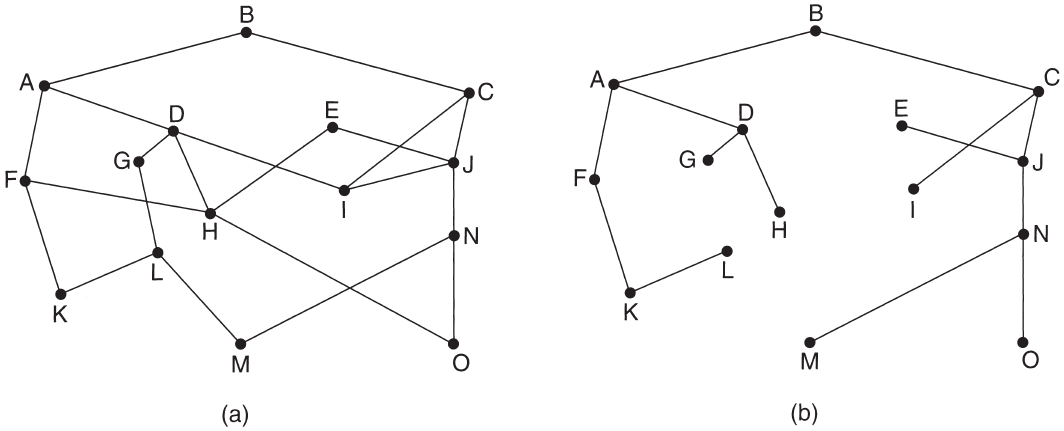
\includegraphics[width=0.5\textwidth-\fboxrule-\fboxrule]{imgs/sumidero.png}}  
\end{wrapfigure}

\textbf{Arbol sumidero:} árbol formado por el grupo de rutas óptimas de todos los orígenes a un destino dado, con raíz en el destino. No contiene ciclos, por lo que cada paquete será entregado en un número de saltos finito y limitado.

La meta de todos los algoritmos de enrutamiento es descubrir y utilizar los árboles sumideros de todos los enrutadores.
\newline

\subsubsection{Enrutamiento por la ruta más corta (algoritmo estático)}

Para elegir una ruta entre un par dado de enrutadores, el algoritmo simplemente encuentra en el grafo la \textbf{ruta más corta} entre ellos. Como determina esta ruta depende de la métrica utilizada. Ver \textbf{Figura 5-7} de [TANEM], página 354, para un ejemplo gráfico del algoritmo.

\subsubsection{Inundación (algoritmo estático)}

Cada paquete de entrada se envía por cada una de las líneas de salida, excepto aquella por la que llegó. Hay que poner medidas para controlar el tráfico infinito de un paquete (por ejemplo, utilizar número de secuencia y un tiempo de vida según un contador de saltos).

Una variación del algoritmo es la \textbf{inundación selectiva}: los enrutadores no envían cada paquete de entrada por todas las líneas, sino \textbf{sólo} por aquellas que van aproximadamente en la dirección correcta. Por lo general, no tiene mucho caso enviar un paquete dirigido al oeste a través de una línea dirigida al este, a menos que la topología sea extremadamente peculiar y que el enrutador esté seguro de este hecho.

La inundación no es práctica en la mayoría de las aplicaciones, pero tiene algunos usos (en el área militar por ejemplo, ante posibles pérdidas múltiples de enrutadores). Siempre escoge la ruta más corta posible, porque escoge en paralelo todas las rutas posibles. En consecuencia, ningún otro algoritmo puede producir un retardo más corto.

\subsubsection{Enrutamiento por vector de distancia (algoritmo dinámico)}

Operan haciendo que cada enrutador mantenga una tabla (es decir, un \textbf{vector}) que da la mejor distancia conocida a cada destino y la línea que se puede usar para llegar ahí. Estas tablas se actualizan intercambiando paquetes de información con los vecinos, que indican la distancia a cada posible destino. Se supone que el enrutador conoce la ``\textit{distancia}" a cada uno de sus vecinos.

Su principal virtud es la sencillez del algoritmo, que permite hacer los cálculos con poca CPU y poca memoria en el enrutador. Es utilizado por el protocolo \textbf{RIP} (\textit{Routing Information Protocol}).

\underline{\textbf{El problema de la cuenta hasta infinito:}}

Este enrutamiento tiene un problema serio en la práctica: aunque llega a la respuesta correcta, podría hacerlo lentamente. En particular, reacciona con rapidez a las buenas noticias, pero con lentitud ante las malas. La \textbf{esencia del problema} consiste en que cuando el enrutador $X$ indica a $Y$ que tiene una ruta en algún lugar, $Y$ no tiene forma de saber si él mismo está en esa ruta.

\begin{figure}[ht!]
  \caption{El problema de la cuenta hasta infinito. Los números indican la distancia en saltos hacia el enrutador $A$. En el caso (a), el enrutador $A$ se activa; en el caso (b), todos los enrutadores están activados y de repente el enrutador $A$ se desactiva.}
  \label{fig:cuenta_infinito}
  \centerline
  {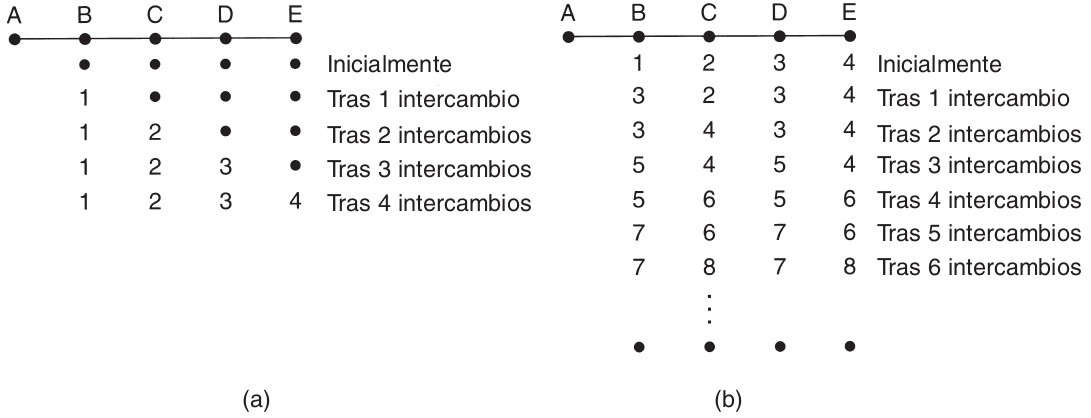
\includegraphics[width=0.9\textwidth-\fboxrule-\fboxrule]{imgs/cuenta_infinito.png}}
\end{figure}

El enrutamiento por vector de distancia es útil cuando se utiliza una métrica sencilla, como por ejemplo el número de saltos, donde el problema de la cuenta hasta infinito es más fácil de resolver.

\subsubsection{Enrutamiento por estado del enlace}

Dos problemas principales causaron la \textbf{desaparición} del \textit{enrutamiento por vector de distancia}: no tomaba en cuenta el ancho de banda al escoger las rutas, y el problema de la cuenta hasta el infinito. Por eso, fue reemplazado por este nuevo tipo de enrutamiento, más fiable y eficiente.

El concepto en el que se basa es sencillo y puede enunciarse en cinco partes. Cada enrutador debe:
\begin{enumerate}
\item Descubrir a sus vecinos y conocer sus direcciones de red.
\item Medir el retardo o costo para cada uno de sus vecinos.
\item Construir un paquete que indique todo lo que acaba de aprender.
\item Enviar este paquete a todos los demás enrutadores.
\item Calcular la ruta más corta a todos los demás enrutadores.
\end{enumerate}

Toda la topología y todos los retardos se miden experimentalmente y se distribuyen a cada enrutador. 

\underline{\textbf{Conocimiento de los vecinos:}}

Cuando un enrutador se pone en funcionamiento, su primera tarea es averiguar quiénes son
sus vecinos; esto lo realiza enviando un paquete \texttt{HELLO} especial a cada línea punto a punto. Se espera que el enrutador del otro extremo regrese una respuesta indicando quién es. Estos nombres deben ser \textbf{globalmente únicos}.

Cuando se conectan dos o más enrutadores mediante una LAN, esta se puede modelar considerandola como otro nodo.

\underline{\textbf{Medición del costo de la línea:}}

El algoritmo requiere que cada enrutador sepa aproximadamente del retardo a cada uno de sus vecinos. La manera más directa de determinar este retardo es enviar un paquete \texttt{ECHO} especial a través de la línea y una vez que llegue al otro extremo, éste debe regresarlo inmediatamente. Al medir el tiempo de ida y vuelta y dividirlo entre dos, el enrutador emisor puede tener una idea razonable del retardo.

La prueba puede llevarse a cabo varias veces y usarse el promedio para mejores resultados. Esto asume de forma implícita que los retardos son \textbf{simétricos}.

Para \textbf{considerar} la carga, el temporizador debe iniciarse cuando el paquete \texttt{ECHO} se ponga en la cola. Para \textbf{ignorar} la carga, el temporizador debe iniciarse cuando el paquete \texttt{ECHO} alcance el frente de la cola.

Para evitar \textbf{oscilaciones} en la selección de la mejor ruta (si se \textit{considera} la carga, ver \textbf{figura 5-12} de [TANEM], página 362), podría ser adecuado dividir la carga entre múltiples líneas, con una fracción conocida de la carga viajando sobre cada una de ellas.

\underline{\textbf{Construcción de los paquetes de estado del enlace:}}

Una vez que se ha recabado la información necesaria para el intercambio, el siguiente paso es que cada enrutador construya un paquete que contenga todos los datos. El paquete comienza con la identidad del emisor, seguida de un número de secuencia, una edad y una lista de vecinos.

Se ha de determinar \textbf{cuándo} construirlos: de manera periódica a intervalos regulares; ó cuando ocurra un evento significativo (caída o reactivación de una línea o de un vecino, por ejemplo).

\underline{\textbf{Distribución de los paquetes de estado del enlace:}}

La idea fundamental es utilizar \textbf{inundación} para distribuir los paquetes de estado del enlace. A fin de mantener controlada la inundación, cada paquete contiene un \textbf{número de secuencia} que se incrementa con cada paquete nuevo enviado. Los enrutadores llevan el registro de todos los pares (\texttt{enrutador de origen, secuencia}) que ven. Cuando llega un paquete de estado del enlace, se verifica contra la lista de paquetes ya vistos. Si es nuevo, se reenvía a través de todas las líneas, excepto aquella por la que llegó. Si es un duplicado, se descarta. Si llega un paquete con número de secuencia menor que el mayor visto hasta el momento, se rechaza como obsoleto debido que el enrutador tiene datos más recientes.

Pueden presentarse algunos problemas:
\begin{enumerate}
\item Los números de secuencia vuelven a comenzar. \textit{Solución}: usar un número de secuencia de \texttt{32 bits}.
\item Si llega a caerse un enrutador, perderá el registro de su número de secuencia. Si comienza nuevamente en 0, se rechazará como duplicado el siguiente paquete.
\item Si llega a corromperse un número de secuencia y se escribe 65,540 en lugar de 4 (un error de \texttt{1 bit}), los paquetes 5 a 65,540 serán rechazados como obsoletos, dado que se piensa que el número de secuencia actual es 65,540.
\end{enumerate}

La solución a estos problemas es incluir la \textbf{edad} de cada paquete después del número de secuencia y disminuirla una vez cada segundo. Cuando la edad llega a cero, se descarta la información de ese enrutador.

Para hacerlo \textbf{más robusto}, una vez que un paquete de estado del enlace llega a un enrutador para ser inundado, no se encola para transmisión inmediata. En vez de ello, entra en un área de almacenamiento donde espera un tiempo breve. Si antes de transmitirlo entra otro paquete de estado del enlace proveniente del mismo origen, se comparan sus números de secuencia. Si son iguales, se descarta el duplicado. Si son diferentes, se desecha
el más viejo.

\underline{\textbf{Cálculo de las nuevas rutas:}}

Una vez que un enrutador ha acumulado un grupo completo de paquetes de estado del enlace, puede construir el grafo de la subred completa porque todos los enlaces están representados. Ahora puede ejecutar localmente el algoritmo de Dijkstra para construir la ruta más corta a todos los destinos posibles. Los resultados de este algoritmo pueden instalarse en las tablas de enrutamiento, y la operación normal puede reiniciarse.

\subsubsection{Enrutamiento jerárquico}

\begin{description}
\item \textbf{Problema:} los algoritmos de enrutamiento no son \textbf{escalables}. La cantidad de información intercambiada aumenta de forma \textbf{no lineal} con el tamaño de la red. En la misma medida aumentan la complejidad de los cálculos, los requerimientos de CPU y memoria en los enrutadores. En cierto momento, la red puede crecer hasta el punto en que ya no es factible que cada enrutador tenga una entrada para cada uno de los
demás enrutadores.
\item \textbf{Solución:} crear \textbf{regiones} (niveles \textit{jerárquicos}), donde cada enrutador conoce todos los detalles para enrutar paquetes a destinos dentro de su propia región, pero no sabe nada de la estructura interna de las otras regiones. Solo algunos enrutadores de cada región comunican con el exterior. Las rutas son menos óptimas, pero se reduce la información de enrutamiento.
\end{description}

\textit{¿Cuántos niveles debe tener la jerarquía?} El número óptimo de niveles para una subred de $N$ enrutadores es de $\ln N$, y se requieren un total de $e \ln N$ entradas por enrutador.

\subsubsection{RIP - Routing Information Protocol}

Protocolo de puerta de enlace interna, que utiliza el protocolo de enrutamiento por \textbf{vector de distancia}.

\begin{wrapfigure}[15]{l}{0.5\textwidth}
  \caption{Formato del paquete RIP.}
  \label{fig:rip_protocol}
  \centering
  \hbox{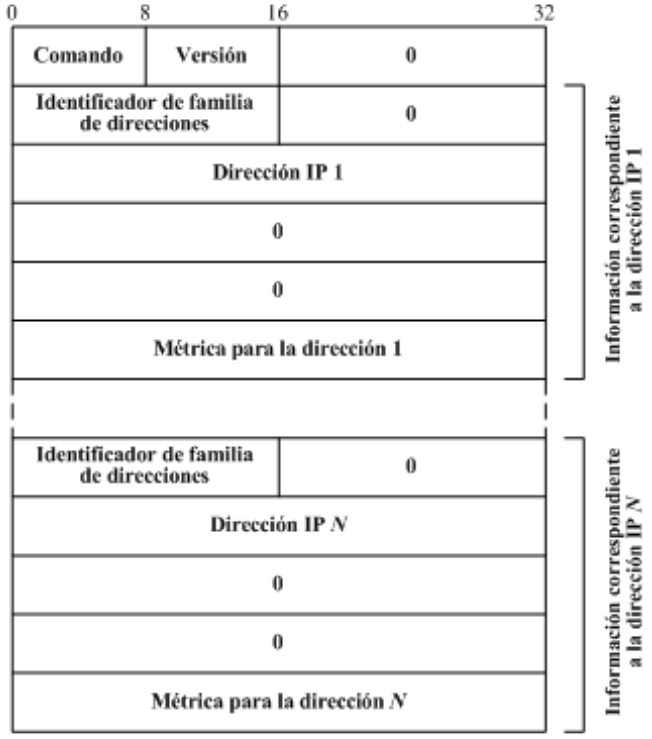
\includegraphics[width=0.5\textwidth-\fboxrule-\fboxrule]{imgs/rip_protocol.png}}
\end{wrapfigure}

\underline{\textbf{Modo de operación:}}

\begin{enumerate}
\item Envía un mensaje a todos sus vecinos, utilizando el puerto 520, pidiendo una copia de la tabla del vecino. El vecino responde con su tabla completa.
\item Cuando esta activo, envía su tabla por \textit{broadcast}, cada 30 seg.
\item ¿Una métrica cambia? $\Rightarrow$ la difunde.
\end{enumerate}

\subsubsection{OSPF - Open Shortest Path First}

Utiliza el protocolo de enrutamiento por \textbf{estado de enlace}. Debe cumplir los siguientes requisitos:
\begin{itemize}
\item Ser abierto (\textit{open}).
\item Ser un algoritmo dinámico.
\item Apoyar una variedad de métricas.
\item Apoyar el enrutamiento con base en el tipo de servicio.
\item Balancear la carga, dividiéndola en líneas múltiples.
\item Implementar un esquema de seguridad.
\end{itemize}

Las categorías utilizadas para \textbf{determinar la métrica} son las siguientes:
\begin{multicols}{2}
\begin{itemize}
\item Normal (\texttt{TOS 0}). Métrica por defecto.
\item  Minimizar el costo monetario (\texttt{TOS 2}).
\item  Maximizar la confiabilidad (\texttt{TOS 4}).
\item  Maximizar el rendimiento real (\texttt{TOS 8}).
\item Minimizar el retardo (\texttt{TOS 15}).
\end{itemize}
\end{multicols}

\begin{wrapfigure}[11]{r}{0.5\textwidth}
  \caption{Formato del paquete OSPF.}
  \label{fig:ospf_protocol}
  \centering
  \hbox{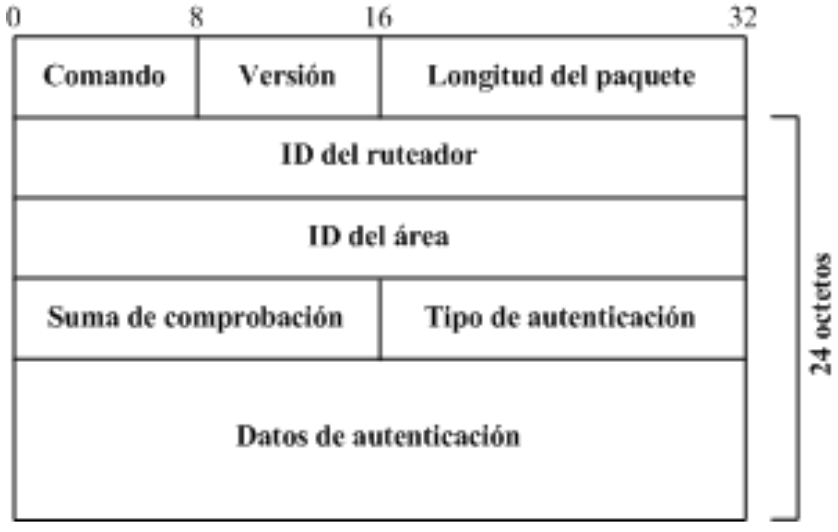
\includegraphics[width=0.5\textwidth-\fboxrule-\fboxrule]{imgs/ospf_protocol.png}}
\end{wrapfigure}

Los \textbf{paquetes} que utiliza son:

\begin{itemize}
\item \texttt{Hello}: Descubre quiénes son los vecinos.
\item \texttt{Link State Update}: Proporciona los costos del emisor a sus vecinos.
\item \texttt{Link State Ack}: Confirma la recepción de la actualización del estado.
\item \texttt{Database Description}: Anuncia qué actualizaciones tiene el emisor.
\item \texttt{Link State Request}: Solicita información del socio.
\end{itemize}

\subsection{Algoritmos de Control de Congestión}

La \textbf{congestión} se produce cuando, al haber demasiados paquetes presentes en la subred (o en una parte de ella), hay una degradación del desempeño. Con mucho tráfico puede que haya incluso una pérdida completa de la capacidad de entregar paquetes (ver \textbf{Figura \ref{fig:congestion}}).

\begin{wrapfigure}{r}{0.5\textwidth}
  \caption{Cuando se genera demasiado tráfico, ocurre congestión y se degrada marcadamente
el desempeño.}
  \label{fig:congestion}  
  \centering
  \hbox{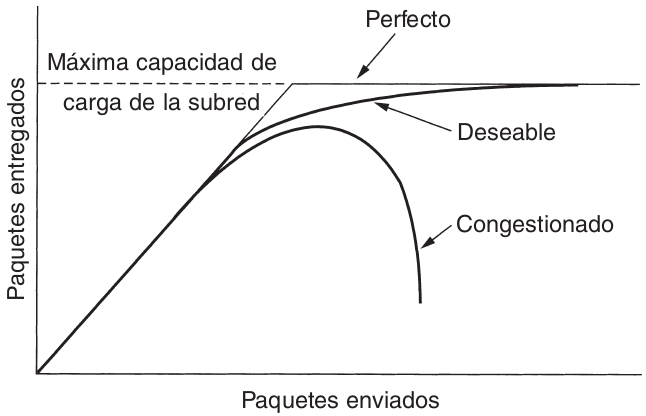
\includegraphics[width=0.5\textwidth-\fboxrule-\fboxrule]{imgs/congestion.png}}  
\end{wrapfigure}

La congestión puede ocurrir por varias razones. Si de manera repentina comienzan a llegar cadenas de paquetes hacia un \textbf{enrutador con varias puertas y una sola salida}, se generará una cola. Si no hay suficiente memoria para almacenar a todos los paquetes, algunos de ellos se descartarán. Incluso con una cantidad infinita de memoria la congestión empeora, ya que para cuando los paquetes llegan al principio de la cola, su temporizador ha terminado (repetidamente) y se han enviado duplicados.

Los \textbf{procesadores lentos}, las líneas de \textbf{poco ancho de banda} y la \textbf{inestabilidad} de enrutadores también pueden causar congestión.
\newline

\underline{\textbf{Control de congestión y control de flujo:}}
\begin{description}
\item \textbf{Control de congestión:} se ocupa de asegurar que la subred sea capaz de transportar el tráfico ofrecido. Es un asunto \textbf{global}, en el que interviene el comportamiento de todos los \textit{hosts}, todos los enrutadores, el proceso de almacenamiento y reenvío dentro de los enrutadores y todos los demás factores que tienden a disminuir la capacidad de transporte de la subred.
\item \textbf{Control de flujo:} se relaciona con el tráfico \textbf{punto a punto} entre un emisor dado y un receptor dado. Su tarea es asegurar que un emisor rápido no pueda transmitir datos de manera continua a una velocidad mayor que la que puede absorber el receptor. Implica normalmente una \textbf{retroalimentación} directa del receptor al emisor.
\end{description}

\subsubsection{Principios generales del control de congestión}

Las redes de computadoras pueden analizarse desde el punto de vista de una \textbf{teoría de control}, que conduce a dividir en \textbf{dos grupos} a todas las soluciones: 

\begin{description}
\item \textbf{Ciclo abierto.} Intentan resolver el problema mediante un buen diseño, para asegurarse en primer lugar de que no ocurra. Una vez que el sistema está en funcionamiento, no se hacen correcciones a medio camino.
Se clasifican entre los que \textbf{actúan en el origen} ó en \textbf{el destino}. Todas toman decisiones \textbf{independientemente} del estado actual de la red.
\item \textbf{Ciclo cerrado.} Se basan en el concepto de un \textbf{ciclo de retroalimentación}. Tiene tres partes:
\begin{enumerate}
\item Monitorear el sistema.
\item Enviar esta información monitoreada.
\item Ajustar la operación del sistema.
\end{enumerate}
Los algoritmos de \textit{ciclo cerrado} se dividen en dos categorías:
\begin{itemize}
\item \textbf{Explícitos.} Regresan paquetes desde el punto de congestión para avisar al origen. 
\item \textbf{Implícitos.} El origen deduce la existencia de una congestión haciendo observaciones locales.
\end{itemize}
\end{description}
\vspace{10pt}
\underline{\textbf{Métricas utilizadas para monitorear la subred en busca de congestiones:}}
\begin{itemize}
\item Porcentaje de paquetes descartados debido a falta de espacio de búfer.
\item Longitud promedio de las colas.
\item Cantidad de paquetes para los cuales termina el temporizador y se transmiten nuevamente.
\item Retardo promedio de los paquetes.
\item Desviación estándar del retardo de paquete.
\end{itemize}

En todos los casos, un \textbf{aumento en las cifras} indica un \textbf{aumento en la congestión}. La presencia de congestión significa que la carga es, \textit{temporalmente}, superior (en una parte del sistema) a la que pueden manejar los recursos.

\subsubsection{Políticas de prevención de congestión}

Los sistemas de \textbf{ciclo abierto} están diseñados para reducir al mínimo la congestión desde el inicio, usando políticas adecuadas en varios niveles (ver \textbf{Figura \ref{fig:politicas_cicloabierto}}).

\begin{figure}[ht!]
  \caption{Políticas relacionadas con la congestión.}  
  \label{fig:politicas_cicloabierto}
  \centerline{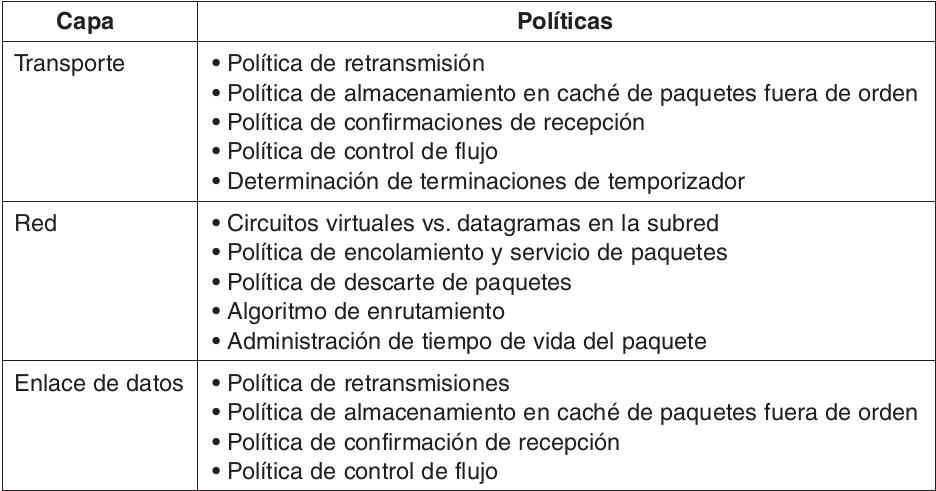
\includegraphics[width=0.8\textwidth-\fboxrule-\fboxrule]{imgs/politicas_cicloabierto.png}}
\end{figure}

\subsubsection{Control de congestión en subredes de CVs}

\underline{\textbf{Control de admisión:}}

Una vez que se ha detectado la congestión, \textbf{no se establecen CVs nuevos} hasta que ha desaparecido el problema.

\begin{wrapfigure}{r}{0.7\textwidth}
  \caption{(a) Subred congestionada. (b) Subred redibujada que elimina la congestión.}
  \label{fig:control_admision}  
  \centering
  \hbox{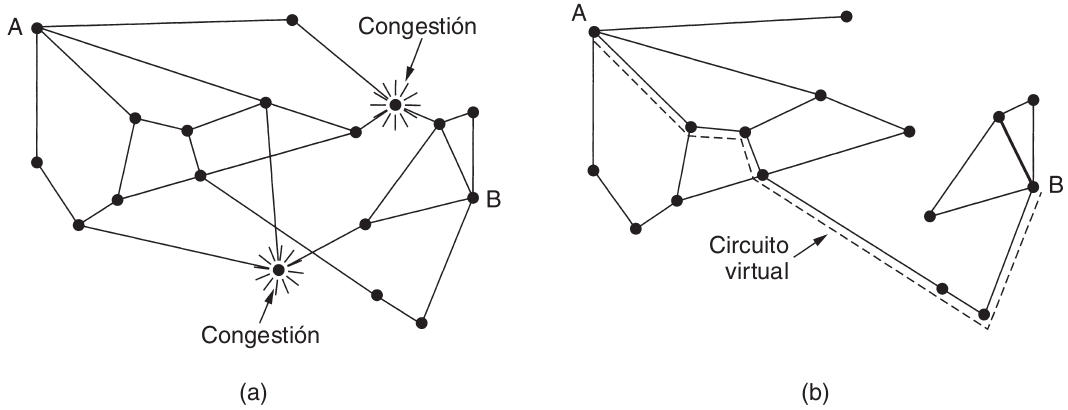
\includegraphics[width=0.7\textwidth-\fboxrule-\fboxrule]{imgs/control_admision.png}}  
\end{wrapfigure}

Un método alterno es \textbf{permitir la creación de nuevos CVs}, pero enrutando cuidadosamente los circuitos nuevos por otras rutas que no tengan problemas (\textbf{Figura \ref{fig:control_admision}}).

Otra estrategia es \textbf{negociar un acuerdo} entre el \textit{host} y la subred cuando se establece un CV. Para cumplir con su parte del acuerdo, la subred reservará recursos a lo largo de la ruta cuando se establezca el circuito. La disponibilidad de todos los recursos necesarios hace poco probable la congestión.

\subsubsection{Control de congestión en subredes de datagramas}

Cada enrutador puede monitorear fácilmente el uso de sus líneas de salida y de otros recursos, por lo que puede elaborar estrategias de control.

\underline{\textbf{El bit de advertencia:}}

Cuando el paquete llega a su destino, la entidad transportadora copia el bit especial (que señala el \textbf{estado de advertencia}) en la siguiente \texttt{ACK} que se regresa al origen. El origen entonces reduce el tráfico.

Mientras el enrutador esté en el estado de advertencia, el bit de advertencia se mantiene activo, y el origen continúa disminuyendo su tasa de transmisión.

\underline{\textbf{Paquetes reguladores:}}

En este método, el enrutador regresa un \textbf{paquete regulador} al \textit{host} de origen, proporcionándole el destino encontrado en el paquete. El paquete original se etiqueta\footnote{Se activa un \texttt{bit} del encabezado.} de manera que no genere más paquetes reguladores. 
Cuando el \textit{host} de origen obtiene el paquete regulador, se le pide que reduzca en un porcentaje $X$ el tráfico enviado al destino especificado.

\underline{\textbf{Paquetes reguladores de salto por salto}}

A altas velocidades o distancias grandes, el envío de un paquete regulador a los \textit{hosts} de origen no funciona bien porque la \textbf{reacción es muy lenta}. Este método hace que el paquete regulador ejerza su efecto en \textbf{cada salto} que da.

Proporciona un alivio rápido al punto de congestión, a expensas de usar más búferes ascendentes. De esta manera puede cortarse la congestión en la raíz, sin que se pierdan paquetes (para representación gráfica, ver \textbf{figura 5-28} de [TANEM], página 393).

\subsubsection{Desprendimiento de carga}

Si el enrutador no puede manejar las cargas, descarta los paquetes y que las
capas superiores se encarguen de enviarlos nuevamente.

Un enrutador abrumado por paquetes simplemente puede escoger paquetes al azar para desprenderse de ellos. Un método alterno es utilizar el descarte según las aplicaciones que se estén ejecutando: en la \textbf{transferencia de archivos} vale más un
paquete viejo que uno nuevo; en \textbf{multimedia} es al revés.

\underline{\textbf{Detección temprana aleatoria:}}

El objetivo es hacer que los enrutadores se deshagan de los paquetes antes de que la situación sea irremediable. Para determinar cuándo comenzar a descartarlos, los enrutadores \textbf{mantienen un promedio móvil} de sus longitudes de cola. Cuando la longitud de cola promedio en algunas líneas sobrepasa un \textit{umbral}, se dice que la línea está congestionada y se toma alguna medida.

\subsubsection{Control de fluctuación}

La \textbf{variación} en el retardo de los paquetes se conoce como \textbf{fluctuación}. Cuando tenemos una fluctuación \textbf{alta} (10[mseg] de diferencia entre paquetes, por ejemplo), se produce un degradado de calidad en las aplicaciones de \textit{streaming} en tiempo real.

La fluctuación puede limitarse calculando el \textbf{tiempo de tránsito esperado} para cada salto en la ruta. Cuando un paquete llega a un enrutador, éste lo examina para saber qué tan adelantado o retrasado está respecto a lo programado. Esta información se almacena en el paquete y se actualiza en cada salto. Si el paquete está adelantado, se retiene durante el tiempo suficiente para regresarlo a lo programado; si está retrasado, el enrutador trata de sacarlo rápidamente.

\subsection{Calidad del Servicio}

El \textbf{flujo} es el conjunto de paquetes que van de un origen a un destino. Se puede caracterizar por cuatro parámetros principales: \textbf{confiabilidad}, \textbf{retardo}, \textbf{fluctuación} y \textbf{ancho de banda}. En conjunto determinan la QoS que el flujo requiere.

En una red \textbf{orientada a la conexión}, todos los paquetes que pertenezcan a un flujo siguen la misma ruta; en una red \textbf{no orientada a la conexión}, pueden seguir diferentes rutas. 

\begin{figure}[ht!]
  \caption{Qué tan rigurosos son los requerimientos de calidad del servicio.}  
  \label{fig:calidad_flujo}
  \centerline{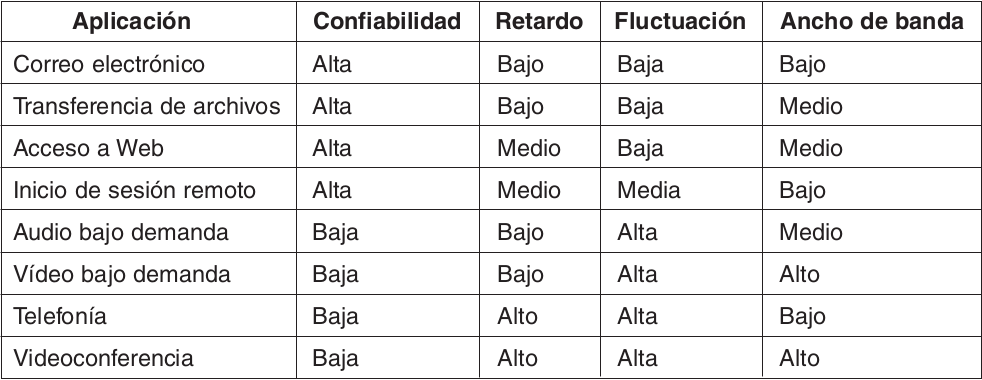
\includegraphics[width=0.8\textwidth-\fboxrule-\fboxrule]{imgs/calidad_flujo.png}}
\end{figure}

\subsubsection{Técnicas para alcanzar una buena calidad de servicio}

Ninguna proporciona QoS eficiente y confiable de una manera óptima. En su lugar, se ha desarrollado una variedad de técnicas, con soluciones prácticas que con frecuencia se combinan múltiples técnicas.

\underline{\textbf{Sobreaprovisionamiento:}}

Proporciona la suficiente capacidad de enrutador, espacio en búfer y ancho de banda como para que los paquetes fluyan con facilidad, a cambio de mayor coste de inversión.

\underline{\textbf{Almacenamiento en búfer:}}

Los flujos pueden almacenarse en el búfer en el lado receptor antes de ser entregados:
\begin{itemize}
\item \textbf{Confiabilidad} y \textbf{ancho de banda}: no les afecta.
\item \textbf{Retardo}: se incrementa.
\item \textbf{Fluctuación}: atenúa o mejora.
\end{itemize}

\underline{\textbf{Modelado de tráfico:}}

Consiste en regular la \textbf{tasa} promedio (y las ráfagas) de la transmisión de los datos. Cuando se establece una conexión, el usuario y la subred acuerdan cierto
patrón de tráfico para ese circuito: forman un \textbf{acuerdo de nivel de servicio}.

El modelado de tráfico \textbf{reduce la congestión}. Para saber si el cliente está cumpliendo con el acuerdo se hace una \textbf{supervisión de tráfico}. Aceptar una forma de tráfico y supervisarlo más tarde es más fácil en las subredes de CVs que en las de datagramas.

Se utiliza para video y audio en tiempo real.

\underline{\textbf{Algoritmo de cubeta con goteo:}}

De manera conceptual, cada \textit{host} está conectado a la red mediante una interfaz que contiene una \textbf{cubeta con goteo} (una cola interna finita). Si llega un paquete cuando la cola está llena, éste se descarta.

\begin{figure}[ht!]
  \caption{(a) Una cubeta con goteo, llena de agua. (b) Cubeta con goteo, llena de paquetes.}
  \label{fig:cubeta_con_goteo}
  \centerline{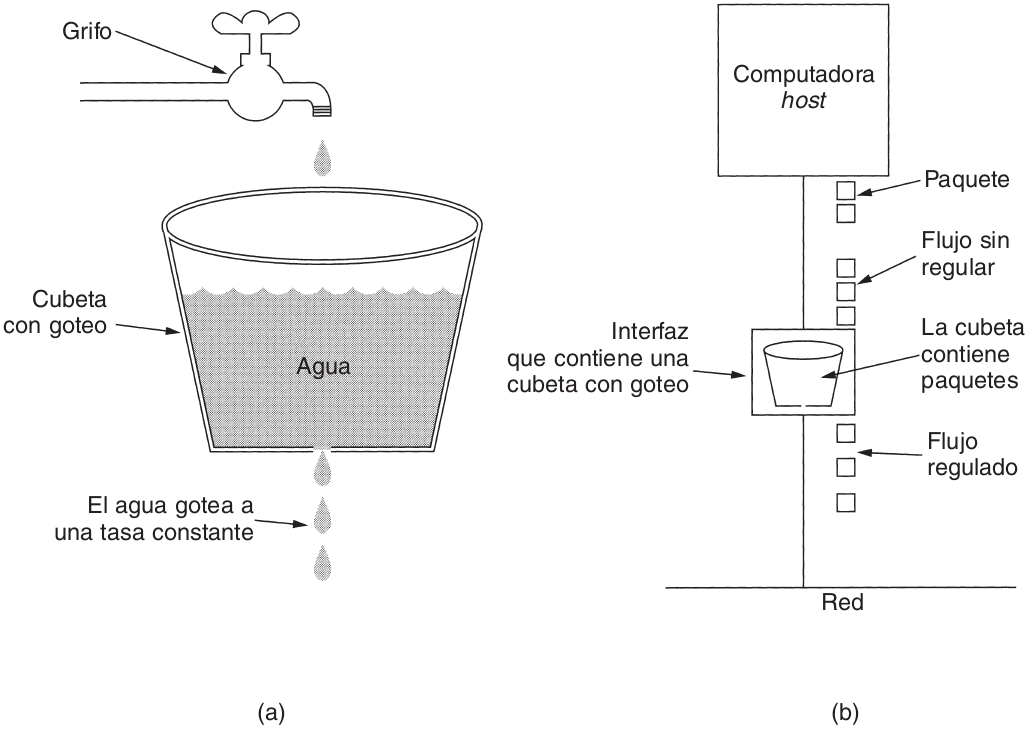
\includegraphics[width=0.8\textwidth-\fboxrule-\fboxrule]{imgs/cubeta_con_goteo.png}}
\end{figure}

Convierte un flujo desigual de paquetes de los procesos de usuario dentro del \textit{host} en un flujo continuo de paquetes hacia la red, moderando las ráfagas y reduciendo las posibilidades de congestión.

\underline{\textbf{Algoritmo de cubeta con \textit{tokens}:}}

El algoritmo de cubeta con goteo impone un patrón de salida rígido a la tasa promedio, sin importar la cantidad de ráfagas que tenga el tráfico. Un algoritmo más flexible puede permitir que la salida se acelere un poco cuando llegan ráfagas grandes.

En esencia, lo que hace este algoritmo es permitir ráfagas, pero limitadas a una longitud máxima regulada. Para ello, funciona con un sistema de permisos (\textit{tokens}).

Los \textit{hosts} inactivos acumulan permisos hasta el tamaño máximo de la cubeta, para enviar posteriormente ráfagas grandes. Esta propiedad proporciona irregularidad en el flujo de salida y da una respuesta más rápida a las ráfagas de entrada repentinas. Cuando se llena la cubeta se descartan \textit{tokens}.

\underline{\textbf{Reservación de recursos:}}

Conociendo una ruta específica para una flujo, es posible reservar recursos a lo largo de esa ruta para asegurar que la capacidad necesaria esté disponible. Estos pueden ser del tipo:
\begin{enumerate}
\item \textbf{Ancho de banda:} no sobrecargar ninguna línea de salida.
\item \textbf{Espacio de búfer:} es posible reservar para que cierto flujo específico no tenga que competir con otros flujos por el espacio en búfer.
\item \textbf{Ciclos de CPU:} el enrutador solo puede procesar cierta cantidad de paquetes por segundo.
\end{enumerate}

\underline{\textbf{Calendarización de paquetes:}}

Si un enrutador maneja múltiples flujos, existe el peligro de que un flujo acapare mucha de su capacidad y limite a los otros flujos.

\begin{description}
\item \textbf{Encolamiento justo.} Los enrutadores tienen colas separadas para cada línea de salida, una por flujo. Cuando una línea se queda inactiva, el enrutador explora las diferentes colas de manera circular, y toma el primer paquete de la siguiente cola. De esta forma, con $n$ \textit{hosts} compitiendo por una línea de salida dada, cada \textit{host} obtiene la oportunidad de enviar uno de $n$ paquetes. El envío de más paquetes no mejorará esta fracción.
\subitem \textbf{Problema:} Proporciona más ancho de banda a los \textit{hosts} que utilizan paquetes más grandes que a los que utilizan paquetes más pequeños.
\subitem \textbf{Solución:} Utilizar exploración circular \texttt{byte} por \texttt{byte} en vez de por paquete.

\item \textbf{Encolamiento justo ponderado.} Permite dar a ciertos \textit{hosts} más ancho de banda que a otros, usando un sistema de prioridades.
\end{description}

\subsubsection{Conmutación de etiquetas y MPLS (MultiProtocol Label Switching}

Para desarrollar mejores métodos de reenvío, se puede agregar una \textbf{etiqueta} en frente de cada paquete y realizar el enrutamiento con base en ella y no con base en la dirección de destino. Hacer que la etiqueta sea un índice de una tabla provoca que encontrar la línea correcta de salida sea una simple cuestión de buscar en una tabla.

\begin{description}
\item \textbf{Enrutamiento:} proceso de buscar una dirección de destino en una tabla para saber a dónde enviar los paquetes hacia ese destino. 
\item \textbf{Conmutación} utiliza una etiqueta que se toma de un paquete como un índice en una tabla de reenvío.
\end{description}

Debido a que los paquetes IP no fueron diseñados para CVs, se tuvo que agregar un nuevo encabezado MPLS en frente del encabezado IP.

\begin{wrapfigure}[12]{r}{0.55\textwidth}
  \caption{Transmisión de un segmento TCP que utiliza IP, MPLS y PPP.}
  \label{fig:mpls_encabezado}
  \centering
  \hbox{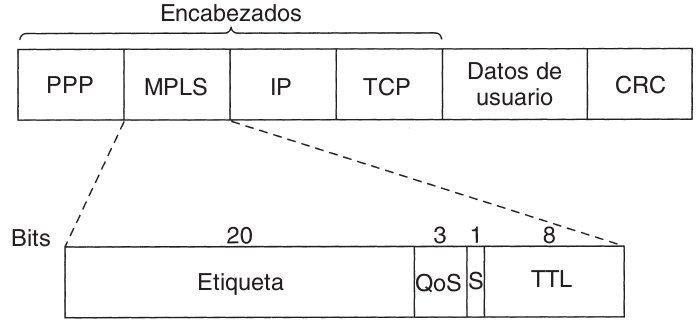
\includegraphics[width=0.55\textwidth-\fboxrule-\fboxrule]{imgs/mpls_encabezado.png}}
\end{wrapfigure}

El encabezado tiene cuatro campos:
\begin{itemize}
\item \textbf{Etiqueta:} contiene los índices.
\item \textbf{QoS:} indica la clase de servicio.
\item \textbf{S}: se relaciona con colocar en una pila múltiples etiquetas en redes jerárquicas.
\item \textbf{TTL:} evita el ciclo infinito en caso de que haya inestabilidad en enrutamiento.
\end{itemize}

Debido a que los encabezados MPLS no son parte del paquete de la CdR o de la trama de la CED, MPLS es en gran medida independiente de ambas capas: es \textbf{multiprotocolo}.

\begin{figure}[ht!]
  \caption{Situación de los protocolos de Internet en el modelo de capas.}
  \label{fig:protocolos_situacion}
  \centerline{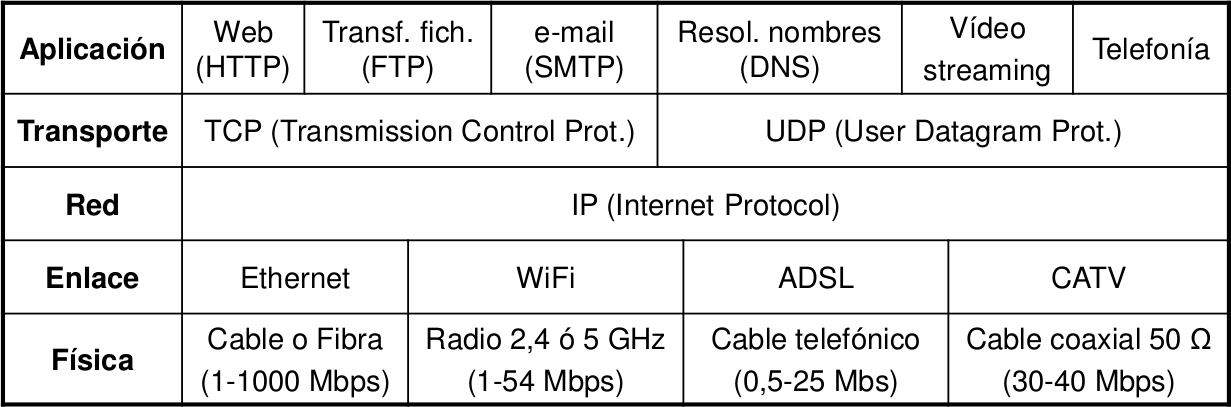
\includegraphics[width=0.85\textwidth-\fboxrule-\fboxrule]{imgs/protocolos_situacion.png}}
\end{figure}

\subsection{La Capa de Red de Internet}

Los principios que guiaron su diseño en el pasado son (del más al menos importante):

\begin{enumerate}
\item \textbf{Asegúrese de que funciona.} No termine el diseño o estándar hasta que múltiples prototipos se hayan comunicado entre sí de manera exitosa.
\item \textbf{Mantenga la simplicidad.} Cuando tenga dudas, utilice la solución más simple.
\item \textbf{Elija opciones claras.} Si hay varias maneras para realizar la misma tarea, elija sólo una.
\item \textbf{Aproveche la modularidad.} Si las circunstancias requieren que un módulo o capa cambie, los otros no se verán afectados.
\item \textbf{Tenga en cuenta la heterogeneidad.} El diseño de la red debe ser simple, general y flexible.
\item \textbf{Evite las opciones y parámetros estáticos.}
\item \textbf{Busque un buen diseño; no es necesario que sea perfecto.} Para manejar algún caso especial, deje que esa parte la resuelvan las personas interesadas en él.
\item \textbf{Sea estricto cuando envíe y tolerante cuando reciba.}
\item \textbf{Piense en la escalabilidad.}
\item \textbf{Considere el desempeño y el costo.}
\end{enumerate}

\subsubsection{El Protocolo IP}

\begin{figure}[ht!]
  \caption{El encabezado de IPv4 (Protocolo Internet).}
  \label{fig:datagrama_ip}
  \centerline{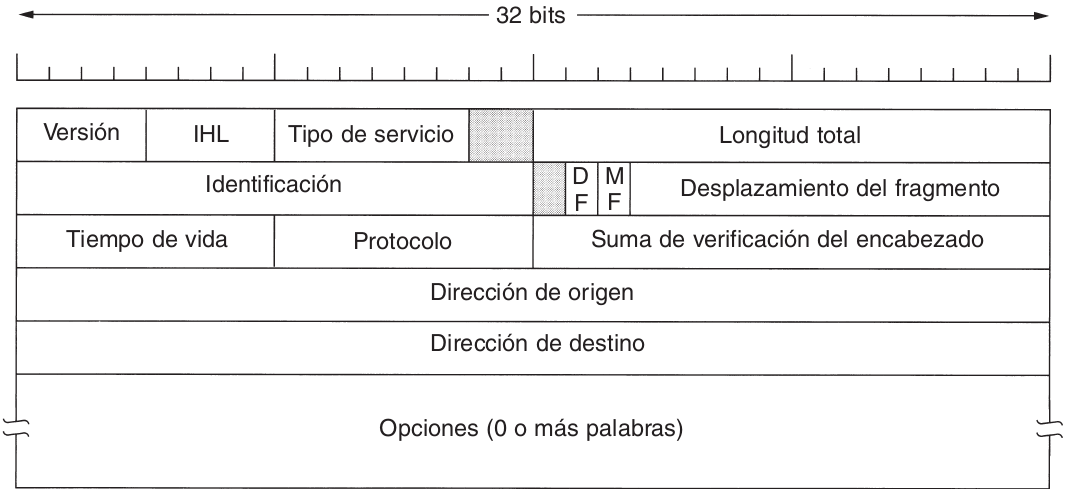
\includegraphics[width=0.85\textwidth-\fboxrule-\fboxrule]{imgs/datagrama_ip.png}}
\end{figure}

El formato de un \textbf{datagrama IP} consiste en una parte de encabezado y una parte de texto. El encabezado tiene una parte fija de \texttt{20 bytes} y una parte opcional de longitud variable. Los  campos son:

\begin{itemize}
\item \textbf{Versión:} siempre vale 4.
\item \textbf{Longitud Cabecera (IHL, \textit{Internet Header Length}):} en palabras de \texttt{32 bits} (rango 5-15).
\item \textbf{Tipo de Servicio:} para \textit{QoS}.
\item \textbf{Longitud total:} expresada en octetos, incluye la cabecera (rango 20-65535)
\item \textbf{Campos de Fragmentación:} Identificación (a qué datagrama pertenece), DF (\textit{Don't Fragment}), MF (\textit{More Fragment}), Desplazamiento del Fragmento (en que parte del datagrama va).
\item \textbf{Tiempo de vida (TTL):} cuenta saltos hacia atrás, se descarta cuando es cero (rango 0-255).
\item \textbf{Protocolo:} indica a que protocolo pertenecen los datos.
\item \textbf{Checksum:} sirve para comprobar la integridad de la cabecera (pero no de los datos).
\item \textbf{Direcciones de origen y destino:} De \texttt{32 bits}, inalteradas durante el TTL del paquete.
\item \textbf{Opciones:} si las hay su longitud debe ser múltiplo de 4 octetos.

\end{itemize}

\begin{figure}[ht!]
  \caption{Algunas de las opciones del datagrama IP.}
  \label{fig:opciones_IP}
  \centerline{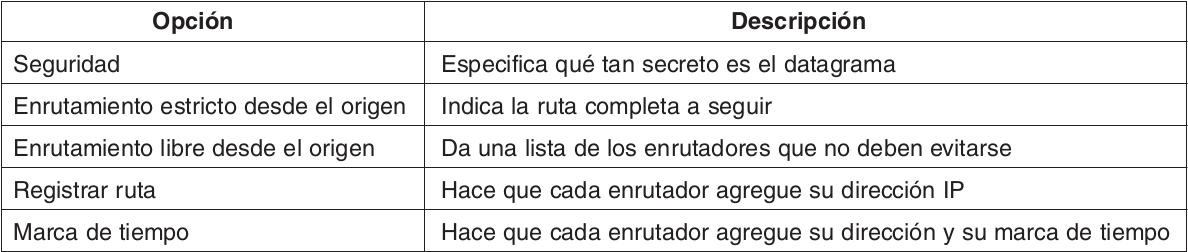
\includegraphics[width=\textwidth-\fboxrule-\fboxrule]{imgs/opciones_IP.png}}
\end{figure}

\subsubsection{Direcciones IP}

Cada \textit{host} y enrutador de Internet tiene una \textbf{dirección IP}, que codifica su número de red y su número de \textit{host}. La combinación es \textbf{única}: no hay dos máquinas que tengan la misma dirección IP. En realidad un dirección IP se refiere a una \textbf{interfaz de red}, no a un \textit{host} en particular.

Las direcciones IP tienen una longitud de 4 \texttt{bytes} (32 \texttt{bits}) y suelen representarse como cuatro números decimales separados por puntos (por ejemplo, 192.168.0.100). El rango máximo va de 0.0.0.0 a 255.255.255.255, aunque algunas direcciones están reservadas:

\begin{itemize}
\item La dirección IP 0.0.0.0 es usada por los \textit{hosts} solo cuando están siendo arrancados. 
\item Las direcciones IP con 0 como número de red se refieren a la red actual (pueden referirse a su propia red sin saber su número).
\item La dirección que consiste solamente en 1s (255) permite la difusión en la red local.
\item Las direcciones con un número de red propio y 255 en el campo de \textit{host} permiten que las máquinas envíen paquetes de difusión a LANs distantes desde cualquier parte de Internet.
\item Por último, todas las direcciones de la forma $127.xx.yy.zz$ se reservan para direcciones locales de prueba (\textit{loopbacks}).
\end{itemize}

Todos los \textit{hosts} de Internet tienen entonces direcciones entre 1.0.0.1 a 223.255.255.254. La asignación de direcciones IP puede hacerse:
\begin{itemize}
\item Por configuración local en el propio equipo.
\item Mediante un protocolo de asignación de direcciones desde un servidor.
\item Utilizando direcciones locales del enlace.
\end{itemize}

Cada interfaz ha de tener asignada una \textbf{máscara}, que indique la longitud del prefijo de red. También se le asigna a cada \textit{host} un \textbf{enrutador por defecto} (\textit{default gateway}), que esté en la misma LAN.

\begin{figure}[ht!]
  \caption{Formatos de dirección IP en \textbf{direccionamiento con clase}. La clase establece donde se sitúa la separación red/\textit{host}.}
  \label{fig:clases_IP}
  \centerline{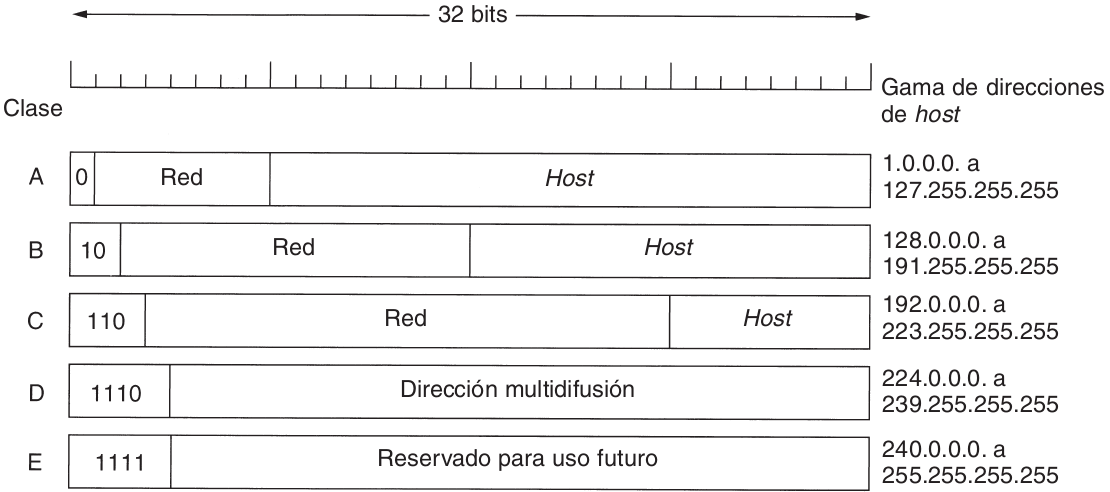
\includegraphics[width=\textwidth-\fboxrule-\fboxrule]{imgs/clases_IP.png}}
\end{figure}

\underline{\textbf{Subredes:}}

Nace de permitir la división de una red en varias partes para uso interno, pero aún actuar como una sola red ante el mundo exterior, para solventar el problema del crecimiento de cantidad de redes. Para hacerlo, algunos \texttt{bits} se eliminan del número de \textit{host} para crear un número de \textbf{subred}.

Para implementar subredes, el enrutador principal necesita una \textbf{máscara de subred} que indique la división entre el número de red + el número de subred y el \textit{host}. Se suele usar una notación ``/$X$'' para indicar que la máscara de subred tiene una longitud de $X$ \texttt{bits}.

\begin{figure}[ht!]
  \caption{Una red clase B dividida en 64 subredes.}
  \label{fig:subred_claseB}
  \centerline{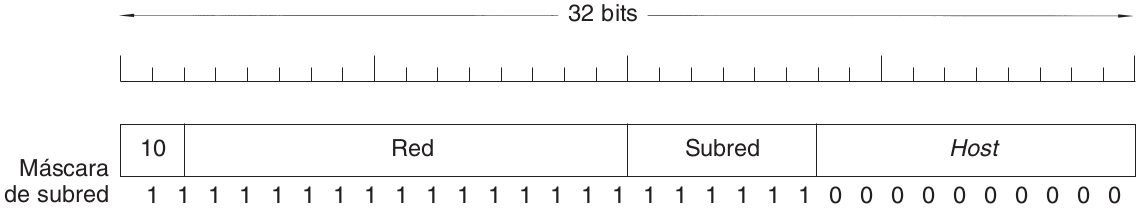
\includegraphics[width=\textwidth-\fboxrule-\fboxrule]{imgs/subred_claseB.png}}
\end{figure}

Cada enrutador tiene una tabla en la que se lista cierto número de direcciones IP (\texttt{red, 0}) y cierto número de direcciones IP (\texttt{esta red, \textit{host}}). El primer tipo indica cómo llegar a redes distantes. El segundo tipo indica cómo llegar a redes locales. \textbf{La interfaz de red a utilizar para alcanzar el destino, así como otra información, está asociada a cada tabla.}

Cuando llega un paquete IP, se busca su dirección de destino en la tabla de enrutamiento. Si el paquete es para una red distante, se reenvía al siguiente enrutador de la interfaz dada en la tabla; si es para un \textit{host} local, se envía directamente al destino. Si la red no está en la tabla, el paquete se reenvía a un enrutador predeterminado con tablas más extensas.

Al introducirse subredes, se cambian las tablas de enrutamiento, agregando entradas con forma de \{\texttt{esta\_red, subred, 0}\} y \{\texttt{esta\_red, esta\_subred, host}\}. Por lo tanto, un enrutador de la subred $k$ sabe cómo llegar a todas las demás subredes y a todos los \textit{hosts} de la subred $k$; no tiene que saber los detalles sobre los \textit{hosts} de otras subredes.

La \textbf{división de redes} reduce entonces espacio en la tabla de enrutamiento creando una jerarquía de tres niveles, que consiste en red, subred y \textit{host}.

\underline{\textbf{CIDR (Classless Inter-Domain Routing):}}

El concepto básico es asignar las direcciones IP en bloques de tamaño variable, \textbf{independientemente de las clases}. Este nuevo esquema se aplica al todo el rango libre de direcciones de las antiguas clases A, B y C (pero no a D, \textit{multicast}, ni E, \textit{reservado}), y hace más complicado el reenvío.

En el nuevo algoritmo implementado por CIDR, cada entrada de tabla de enrutamiento se extiende para darle una máscara de \texttt{32 bits}. De esta manera, ahora hay una sola tabla de enrutamiento para todas las redes que consten de un arreglo de tres variables \{\texttt{dirección IP}, \texttt{máscara de subred}, \texttt{línea saliente}\}. Cuando llega un paquete, primero se extrae su dirección de destino IP. Luego (\textit{conceptualmente}) se analiza la tabla de enrutamiento entrada por entrada, enmascarando la dirección de destino y comparándola con la entrada de la tabla buscando una correspondencia. Es posible que coincidan entradas múltiples (con diferentes longitudes de máscara de subred), en cuyo caso se usa la máscara más larga. De esta manera, si hay una coincidencia para una máscara /20 y una máscara /24, se usa la entrada /24.


\subsubsection{Protocolos de Control en Internet}

Además del IP que se usa para transferencia de datos, Internet tiene algunos protocolos de control que se usan en la CdR:
\begin{itemize}
\item \textbf{ICMP (Internet Control Message Protocol)}: mensajes de error y situaciones anómalas.
\item \textbf{ARP}: Resolución de direcciones MAC.
\item \textbf{RARP, BOOTP, DHCP}: Resolución de direcciones IP.
\item \textbf{IGMP}: Gestión de grupos \textit{multicast}.
\end{itemize}

\underline{\textbf{ICMP - Protocolo de Mensajes de Control de Internet:}}

Permite reportar diversas incidencias o situaciones excepcionales que pueden producirse en el envío de un datagrama. Todos los mensajes ICMP se envían en datagramas IP (1 en el campo \textit{protocolo}). Generalmente los mensajes ICMP incluyen como datos la \textbf{cabecera} y los primeros bytes de datos del paquete que ha provocado el mensaje ICMP.

\begin{tabular}{p{4cm} p{11 cm}}
{\bf Mensaje} & {\bf Significado} \\\hline \\ [-1.5ex]
\textit{Destination Unreachable}

(Destino inaccesible)
& Red, \textit{host}, protocolo o puerto inaccesible o desconocido. 

Datagrama demasiado grande que tiene prohibida la fragmentación (\texttt{bit DF} puesto).
\\ [1ex] \hline \\ [-1.5ex]
\textit{Source Quench}

(Apagar la fuente)
& Ejerce \textbf{control de flujo} sobre el emisor en casos de congestión. No se utiliza. Actualmente se realiza el control de congestión de forma implícita, sin envío de mensajes explícitos.
\\ [1ex] \hline \\ [-1.5ex]
\textit{Echo Request}, y

\textit{Echo Reply}
& Sirve para comprobar la accesibilidad de la IP remota (comando usado: \texttt{ping}).
\\ [1ex] \hline \\ [-1.5ex]
\textit{Time Exceeded}

(Tiempo excedido)
& Datagrama descartado por agotamiento del \texttt{TTL} (comando usado: \texttt{traceroute}).
\\ [1ex] \hline \\ [-1.5ex]
\textit{Redirect}

(Cambio de ruta)
& El enrutador nos sugiere un camino mejor que el que estamos utilizando (más corto).
\\ [1ex] \hline \\ [-1.5ex]
\end{tabular}

\underline{\textbf{ARP - Protocolo de Resolución de Direcciones:}}

¿\textit{Cómo se convierten direcciones IP en direcciones de CED}? El \textbf{Protocolo de Resolución de Direcciones (ARP)} lo que hace es preguntar al resto de su LAN quién posee la dirección IP destino, y la máquina destino le responde con su dirección de CED. Cuando la dirección destino se encuentra fuera de la LAN, el ARP de la máquina origen lo buscará usando el enrutador.

La ventaja de usar ARP en lugar de archivos de configuración -que relacionan direcciones IP con direcciones de CED- es la \textbf{sencillez}.

\underline{\textbf{RARP, BOOTP y DHCP:}}

\begin{description}
\item \textbf{RARP (\textit{Reverse ARP}).} A partir de una dirección Ethernet, devuelve la dirección IP correspondiente.
\item \textbf{BOOTP (\textit{Bootstrap Protocol}).} Reemplazo de RARP. Usa mensajes UDP que envía a través de los enrutadores. Además proporciona otra información adicional además de la dirección IP.
\item \textbf{DHCP (\textit{Dynamic Host Configuration Protocol}).} BOOTP extendido. Permite asignación de IP manual y automática (BOOTP sólo permite manual).
\end{description}

\section{La Capa de Transporte}

Es el corazón de toda la jerarquía de protocolos. Su tarea es la de proporcionar un transporte de datos \textbf{confiable} y \textbf{económico} de la máquina de origen a la máquina de destino, independientemente de la red o redes físicas en uso.

\subsection{El Servicio de Transporte}

\underline{\textbf{Servicios proporcionados a las capas superiores:}}

La meta fundamental es proporcionar un servicio \textbf{eficiente}, \textbf{confiable} y \textbf{económico} a sus usuarios (normalmente procesos de la CdA). Para ello, utiliza los servicios proporcionados por la CdR. El HW o SW de la CdT que se encarga del trabajo se llama \textbf{entidad de transporte}.

Ofrece dos tipos de servicios, los cuales son muy parecidos a sus homónimos en la CdR:
\textbf{orientado} y \textbf{no orientado a la conexión.} 

La diferencia entre los servicios proporcionados por la CdR y por la CdT es en \textbf{dónde se ejecuta el código de transporte}; en el primero es en los \textbf{enrutadores}, mientras que en el segundo es en los \textit{\textbf{hosts}}.

Esencialmente, la existencia de la CdT hace posible que el \textbf{servicio de transporte} sea \textbf{más confiable} que el \textbf{servicio de red} subyacente, ya que puede detectar y compensar paquetes perdidos y datos alterados. 

La CdT cumple la función clave de \textbf{aislar} a las capas superiores de la tecnología, el diseño y las imperfecciones de la subred. De esta manera, se hace la distinción: las cuatro capas del 1 al 4 pueden verse como el \textbf{proveedor del servicio de transporte}, y el resto de las capas superiores son el \textbf{usuario del servicio de transporte}.

\subsubsection{Primitivas del servicio de transporte}

La \textbf{esencia} del \textbf{servicio de transporte orientado a la conexión} es ocultar las imperfecciones del servicio de red para que los procesos usuarios puedan dar por hecho simple mente la existencia de un flujo de \texttt{bits} libre de errores.

Una diferencia entre los servicios de red y de transporte es a quién están dirigidos: el primero lo usan únicamente las entidades de transporte; al segundo lo usan muchos programas (por lo que debe ser adecuado y fácil de usar).

\begin{figure}[ht!]
  \caption{Anidamiento de las TDPUs, los paquetes y las tramas.}
  \label{fig:anidamiento}
  \centerline{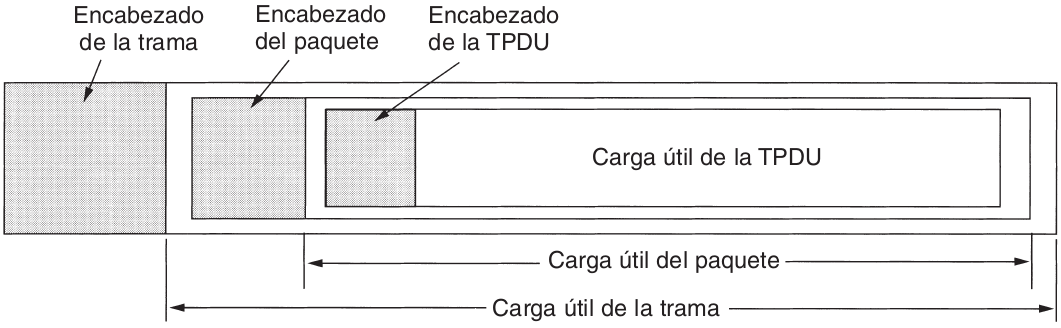
\includegraphics[width=0.95\textwidth-\fboxrule-\fboxrule]{imgs/anidamiento.png}}
\end{figure}

\textbf{TDPU (Unidad de Datos del Protocolo de Transporte)} hace referencia a los mensajes enviados de una entidad de transporte a otra.

\begin{figure}[ht!]
  \caption{Primitivas de un servicio de transporte sencillo.}
  \label{fig:primitivas_transporte}
  \centerline{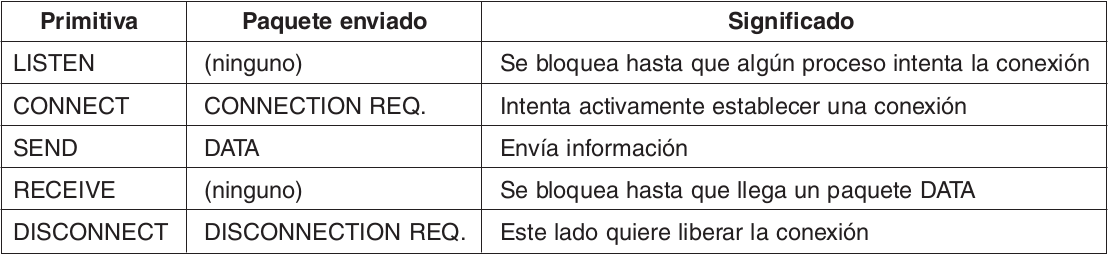
\includegraphics[width=0.95\textwidth-\fboxrule-\fboxrule]{imgs/primitivas_transporte.png}}
\end{figure}

Proceso en capa de transporte:
\begin{enumerate}
\item El servicio ejecuta una primitiva \texttt{LISTEN}.
\item Un cliente quiere conectarse a un servidor y ejecuta una primitiva \texttt{CONNECT}.
\item El \texttt{CONNECT} invoca a una TDPU \texttt{CONNECTION REQUEST} al servidor.
\item El servidor envía una TDPU \texttt{CONNECTION ACCEPTED}.
\item Ahora los datos se envían usando las primitivas \texttt{SEND} y \texttt{RECEIVE}.
\item Cuando ya no se necesitan una conexión se emite un TDPU \texttt{DISCONNECT}.
\end{enumerate}

\begin{figure}[ht!]
  \caption{Diagrama de estado de un esquema sencillo de manejo de conexiones. Las transiciones escritas en cursivas son causadas por llegadas de paquetes. Las líneas continuas muestran la secuencia de estados del cliente. Las líneas punteadas muestran la secuencia de estados del servidor.}
  \label{fig:digrama_estado_TDPU}
  \centerline{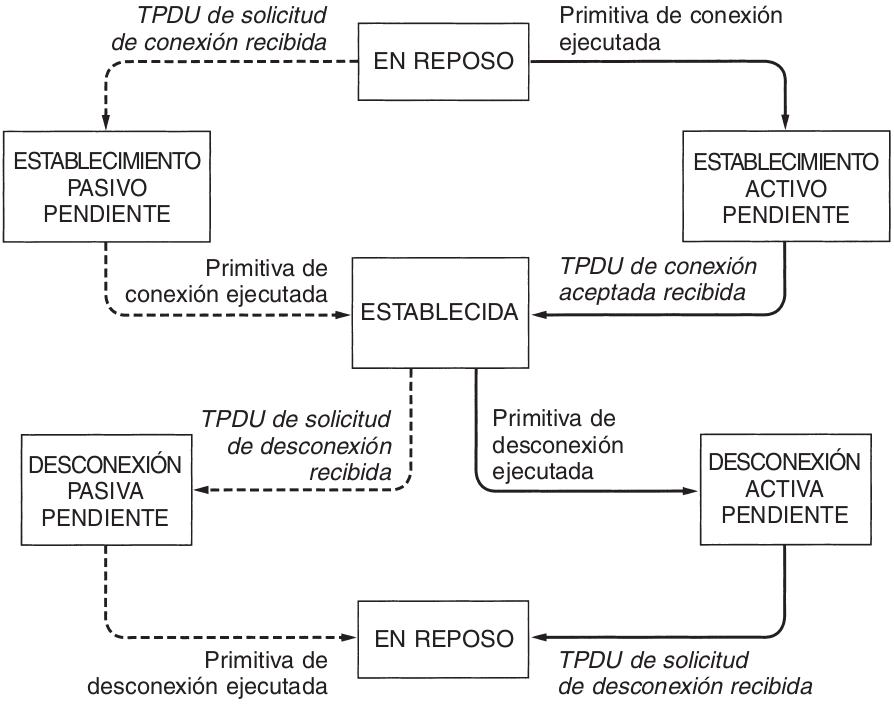
\includegraphics[width=0.8\textwidth-\fboxrule-\fboxrule]{imgs/digrama_estado_TDPU.png}}
\end{figure}

\subsection{Elementos de los Protocolos de Transporte}

El servicio de transporte se implementa mediante un \textbf{protocolo de transporte} entre las dos entidades de transporte. Este se encarga del control de errores, la secuenciación y el control de flujo, entre otros aspectos.

\underline{\textbf{Diferencias entre los servicios protocolos de cada capa:}}

\begin{tabular}{p{7.5cm}p{7.5cm}}
{\bf Capa de Enlace} & {\bf Capa de Transporte} \\\hline \\ [-1.5ex]
No es necesario direccionamiento.
&
Se requiere saber la dirección destino.
\\ [1ex] \hline \\ [-1.5ex]
Establecimiento de la conexión sencillo.
&
Establecimiento de la conexión complejo.
\\ [1ex] \hline \\ [-1.5ex]
No existe capacidad de almacenamiento entre los enrutadores.
&
Existe la posibilidad que los paquetes queden almacenados en la subred durante un tiempo finito.
\\ [1ex] \hline \\ [-1.5ex]
Se necesitan búferes.
&
Se necesitan búferes pero de mayor capacidad.
\\ [1ex] \hline \\ [-1.5ex]
\end{tabular}

\subsubsection{Direccionamiento}

El método que normalmente se emplea es definir direcciones de transporte en las que los procesos pueden estar a la escucha de solicitudes de conexión. En Internet, estos puntos terminales se denominan \textbf{puertos}; acá usamos el término genérico \textbf{TSAP} (\textbf{Punto de Acceso al Servicio de Transporte}). Los puntos terminales análogos de la CdR se llaman \textbf{NSAP} (\textbf{Punto de Acceso al Servicio de Red}) (\textit{las direcciones IP son ejemplos de NSAPs}).

\begin{wrapfigure}[20]{r}{0.55\textwidth}
  \caption{TSAPs, NSAPs y conexiones de transporte.}
  \label{fig:tsap_nsap}
  \centerline{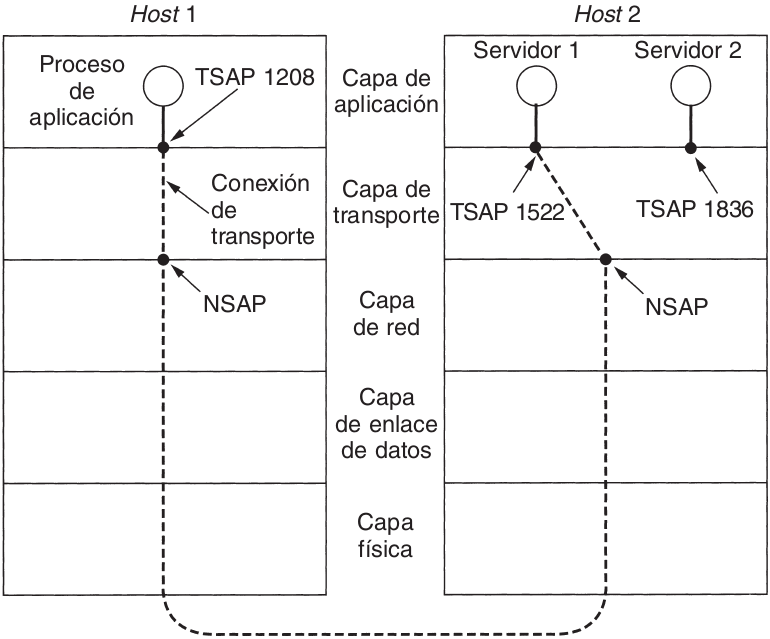
\includegraphics[width=0.55\textwidth-\fboxrule-\fboxrule]{imgs/tsap_nsap.png}}
\end{wrapfigure}

Como en algunas redes cada computadora tiene un solo NSAP, los TSAPs sirven para distinguir los múltiples puntos terminales de transporte que comparten un NSAP.

\underline{\textbf{Protocolo inicial de conexión:}}

En lugar de que cada servidor concebible escuche en un TSAP bien conocido, cada máquina que desea ofrecer servicio a usuarios remotos tiene un \textbf{servidor de procesos} especial que actúa como \textit{proxy} de los servidores de menor uso. Este servidor escucha en un grupo de puertos al mismo tiempo, esperando una solicitud de conexión.

En un esquema alterno existe un proceso especial llamado \textbf{servidor de nombres}. Para encontrar la dirección TSAP correspondiente a un nombre de servicio dado, el usuario establece una conexión con el servidor de nombres (que escucha en un TSAP bien conocido). Entonces el usuario envía un mensaje especificando el nombre del servicio, y el servidor de nombres devuelve la dirección TSAP. Luego el usuario libera la conexión con el servidor de nombres y establece una nueva con el servicio deseado.

\subsubsection{Establecimiento de una conexión}

El establecimiento de una conexión se complica dada la \textbf{existencia de duplicados retrasados}. Si podemos asegurar que ningún paquete viva más allá de cierto tiempo conocido, el problema se vuelve algo más manejable.

El tiempo de vida de un paquete puede restringirse a un máximo conocido usando:
\begin{enumerate}
\item Un diseño de subred restringido.
\item Colocar un contador de saltos en cada paquete.
\item Marcar el tiempo en cada paquete.
\end{enumerate}

\underline{\textbf{Acuerdo de tres vías:}}

Este protocolo de establecimiento no requiere que ambos lados comiencen a transmitir con el mismo número de secuencia, por lo que puede usarse con otros métodos de sincronización distintos del método de reloj global.

\begin{figure}[ht!]
  \caption{Tres escenarios para establecer una conexión usando un acuerdo de tres vías. CR significa \texttt{CONNECTION REQUEST}. (a) Operación normal. (b) \texttt{CONNECTION REQUEST} duplicada vieja que aparece de la nada. (c) \texttt{CONNECTION REQUEST} duplicada y \texttt{ACK} duplicada.}
  \label{fig:acuerdo_tres_vias}
  \centerline{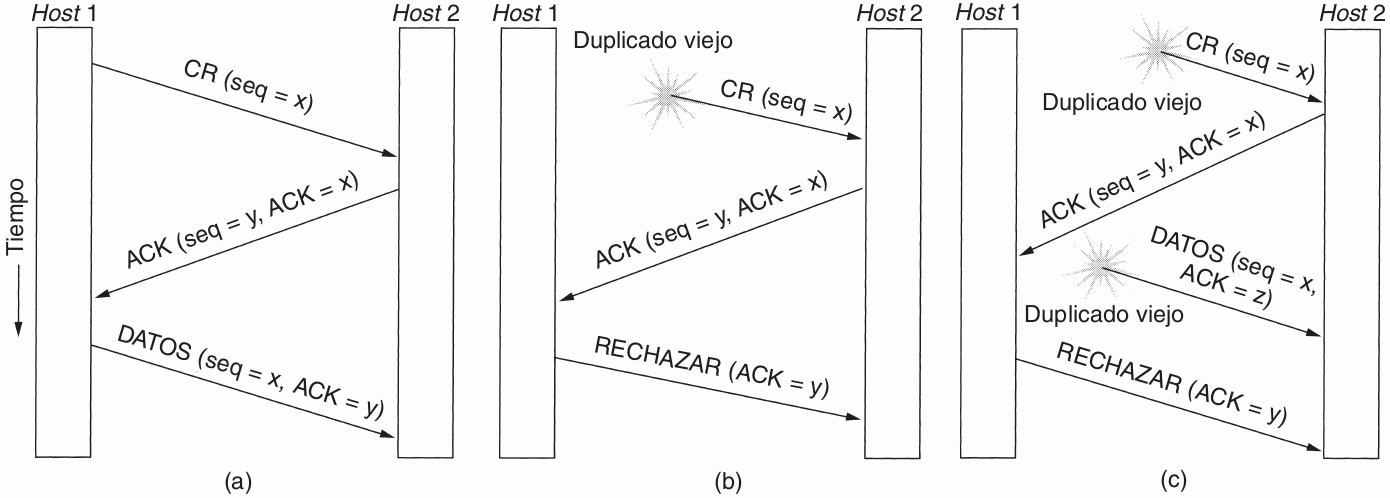
\includegraphics[width=\textwidth-\fboxrule-\fboxrule]{imgs/acuerdo_tres_vias.png}}
\end{figure}

El procedimiento normal de establecimiento al iniciar el \textit{host 1} (ver \textbf{Figura \ref{fig:acuerdo_tres_vias}}). El \textit{host 1} escoge un número de secuencia, $x$, y envía al \textit{host 2} una TDPU \texttt{CONNECTION REQUEST} que lo contiene. El \textit{host 2} responde con una TDPU \texttt{CONNECTION ACCEPTED} confirmando la recepción de $x$ y anunciando su propio número de secuencia inicial, y. Por último, el \textit{host 1} confirma la recepción de la selección de un número de secuencia inicial del \textit{host 2} en la primera TDPU de datos que envía.

\begin{wrapfigure}[17]{r}{0.45\textwidth}
  \caption{Desconexión abrupta con pérdida de datos (asimétrica).}
  \label{fig:liberacion_asimetrica}
  \centering
  \hbox{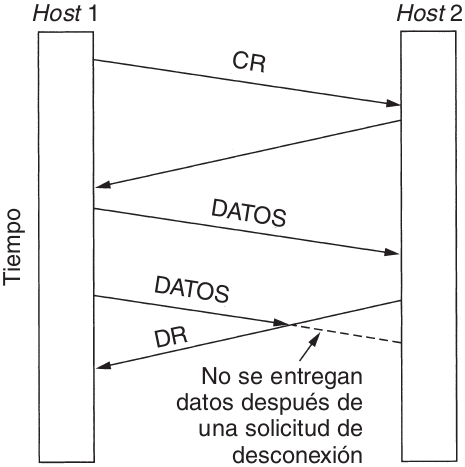
\includegraphics[width=0.35\textwidth-\fboxrule-\fboxrule]{imgs/liberacion_asimetrica.png}}
\end{wrapfigure}

\subsubsection{Liberación de una conexión}

Existen dos formas de liberar una conexión:

\begin{itemize}
\item \textbf{Liberación asimétrica.} Cuando una parte cuelga, se interrumpe la conexión. Es abrupta y puede resultar en la pérdida de datos (ver \textbf{Figura \ref{fig:liberacion_asimetrica}}.
\item \textbf{Liberación simétrica.} Trata la conexión como dos conexiones unidireccionales distintas, y requiere que cada una se libere por separado. Es ideal cuando cada proceso tiene una cantidad fija de datos por enviar y sabe con certidumbre cuándo los ha enviado. Sin embargo, tiene el \textbf{problema de los dos ejércitos}.
\end{itemize}

\underline{\textbf{Problema de los dos ejércitos:}}

Esencialmente, no importa cuántas rondas de confirmación se lleven a cabo, no hay forma de garantizar que ambos \textit{hosts} coincidan en que la \textbf{solicitud de desconexión} ha sido entregada y que no se haya alterado o perdido alguna de las solicitudes entre medio.

Para tratar de solucionarlo en parte se agregan \textbf{temporizadores} que expiran luego de cierto tiempo (ver \textbf{Figura \ref{fig:liberacion_simetrica}}). Aunque este protocolo puede fallar si se pierden tanto la \texttt{DR} y se suceden $N$ retransmisiones: el emisor se dará por vencido y liberará la conexión, mientras el otro lado nunca se enterará de esto y mantendrá la conexión (situación de \textbf{conexión semiabierta}). 

Hay soluciones que arreglan algunos de estos problemas, pero generan otros: \textit{no hay un protocolo perfecto}.
\newline
\begin{figure}[ht!]
  \caption{Cuatro escenarios de un protocolo para liberar una conexión. (a) Caso normal del acuerdo de tres vías. (b) Pérdida de la última \texttt{ACK}. (c) Respuesta perdida. (d) Respuesta perdida y pérdida de las \texttt{DRs} subsecuentes.}
  \label{fig:liberacion_simetrica}
  \centerline{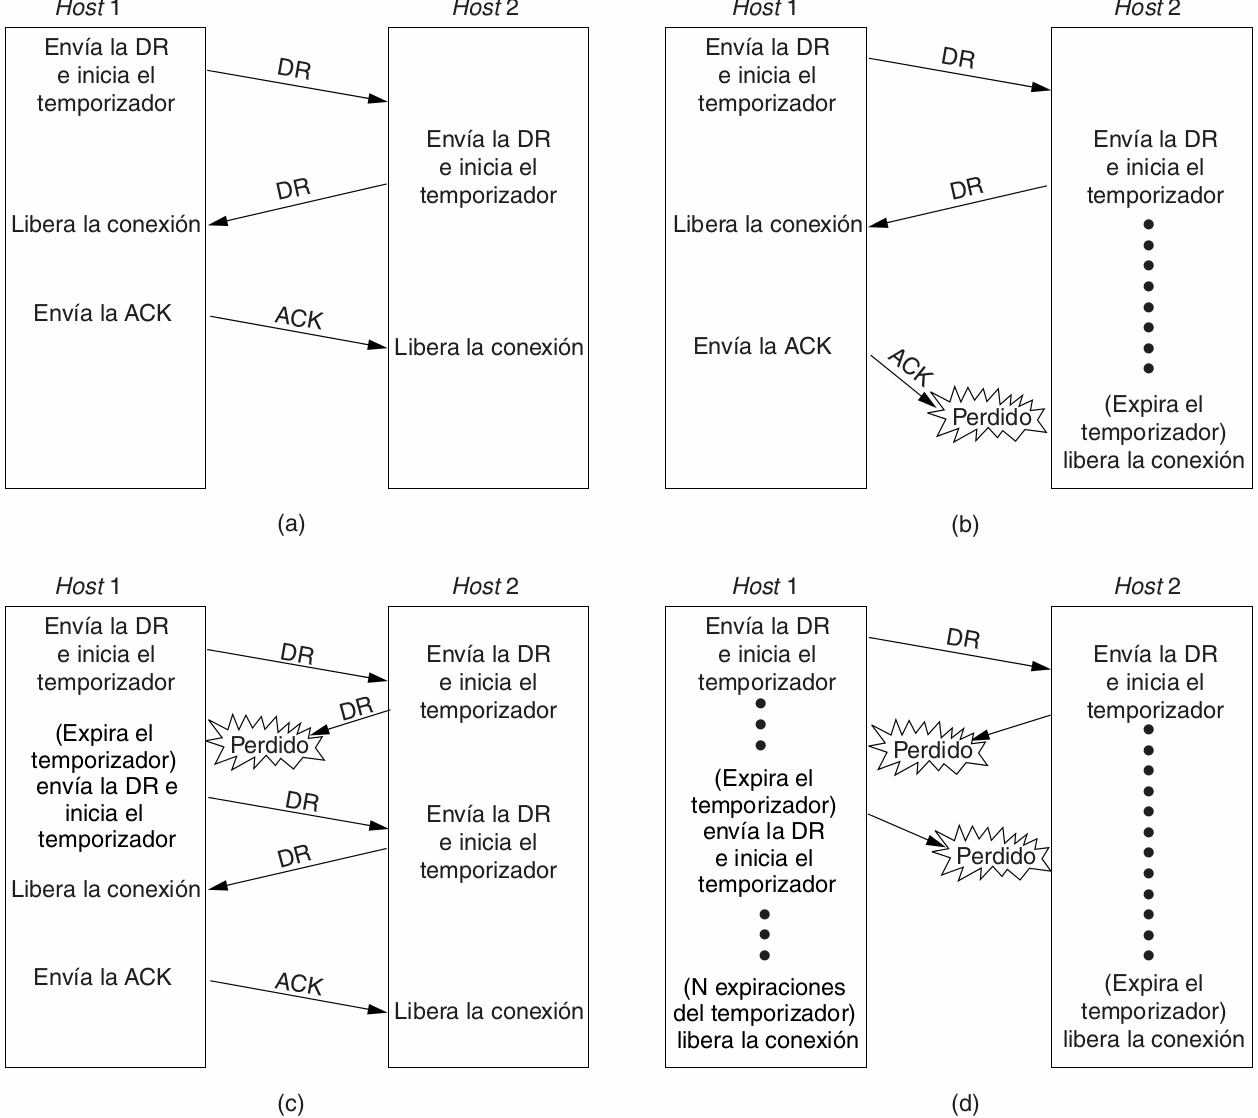
\includegraphics[width=\textwidth-\fboxrule-\fboxrule]{imgs/liberacion_simetrica.png}}
\end{figure}

\subsubsection{Control de flujo y almacenamiento en búfer}

En algunos sentidos el problema del \textbf{control de flujo} en la CdT es igual que en la CED, pero en otros es diferente. Ambas capas se requiere una \textbf{ventana corrediza} u otro esquema en cada conexión para evitar que un emisor rápido desborde a un receptor lento. La diferencia principal es que un enrutador por lo regular tiene relativamente pocas líneas, y que un \textit{host} puede tener numerosas conexiones. 

Si el servicio de red es \textbf{no confiable}, el emisor debe almacenar en búfer todas las TDPUs enviadas, igual que en la CED.

Si el servicio de red es \textbf{confiable}, se pueden hacer otros arreglos. El receptor no puede garantizar que se aceptará cada TDPU que llegue, por lo que tendrá el emisor que usar búferes. Además el emisor no puede confiar en la ACK de la CdR porque esto sólo significa que ha llegado la TDPU, no que ha sido aceptada. La cuestión está en determinar el tamaño de los búferes en el receptor. En la \textbf{Figura \ref{fig:buferes_dinamicos}} pueden verse distintos acercamientos.

\begin{figure}[ht!]
  \caption{(a) Búferes encadenados de \textbf{tamaño fijo}: ideal al tener TDPUs del mismo tamaño, ineficiente en otro caso. (b) Búferes encadenados de \textbf{tamaño variable}: mejor uso de memoria a coste de mayor complejidad de administración. (c) Un gran búfer \textbf{circular} por conexión: eficiente solo en carga alta.}
  \label{fig:buferes_dinamicos}
  \centerline{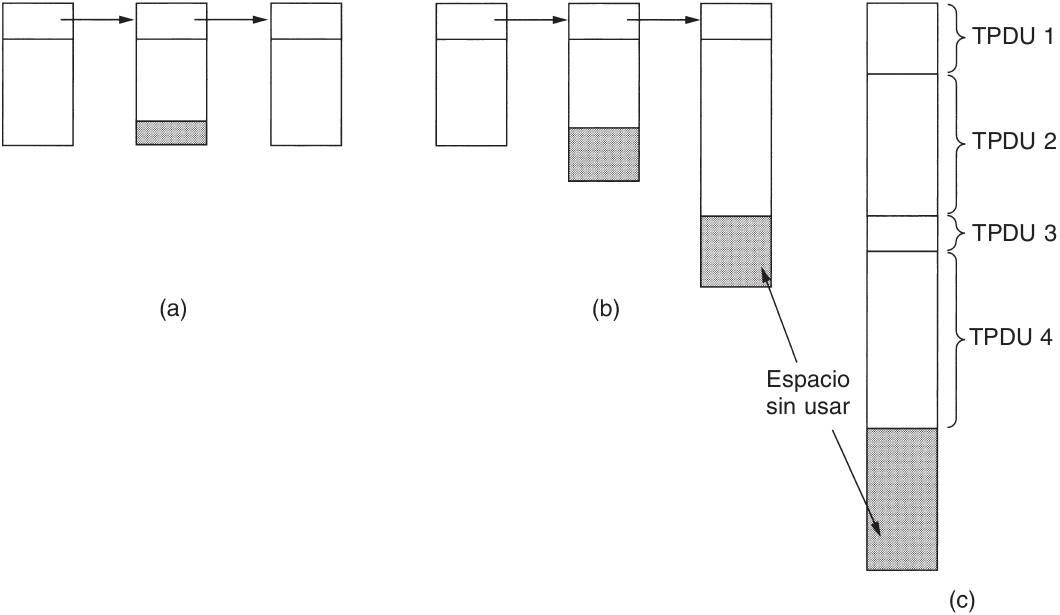
\includegraphics[width=\textwidth-\fboxrule-\fboxrule]{imgs/buferes_dinamicos.png}}
\end{figure}

El \textbf{equilibrio óptimo} entre el almacenamiento en búfer en el origen y en el destino depende del tipo de tráfico transportado por la conexión: para un tráfico en ráfagas de bajo ancho de banda, es mejor mantener búferes en el emisor; para tráfico continuo de alto ancho de banda, es mejor hacerlo en el receptor.

\underline{\textbf{Manejando la asignación dinámica de buffer:}}

Además de necesitar una \textbf{ventana de tamaño variable}, se usa el siguiente procedimiento de asignación:
\begin{enumerate}
\item El emisor solicita una cierta cantidad de búferes.
\item El receptor otorga tantos búferes como puede. Cada vez que el emisor envía una TDPU, disminuye su asignación, deteniéndose por completo al llegar la asignación a cero.
\item El receptor entonces incorpora tanto las ACKs como las asignaciones de búfer al tráfico de regreso.
\end{enumerate}

Para evitar una situación de \textbf{bloqueo irreversible} al perderse una TDPU de control, cada \textit{host} debe enviar periódicamente una TDPU de control con la ACK y estado de búferes de cada conexión.

\underline{Nota:} Si llegase un momento en que el espacio de búfer dejase de limitar el flujo máximo, se necesitará un mecanismo basado por otro lado en la \textbf{capacidad de carga} de la subred. Como por ejemplo, de ventana corrediza cuyo tamaño de ventana emisora depende de este parámetro.

\subsubsection{Multiplexión}

Existen dos tipos de multiplexión en la CdT:
\begin{description}
\item \textbf{Hacia arriba.} Cuando llega un TDPU, se necesita algún mecanismo para saber a cual proceso asignarla.
\item \textbf{Hacia abajo.} Si un usuario necesita más ancho de banda del que le puede proporcionar un CV, una alternativa es abrir múltiples conexiones de red y distribuir el tráfico entre ellas.
\end{description}

\begin{figure}[ht!]
  \caption{(a) Multiplexión hacia arriba. (b) Multiplexión hacia abajo.}
  \label{fig:multiplexion}
  \centerline{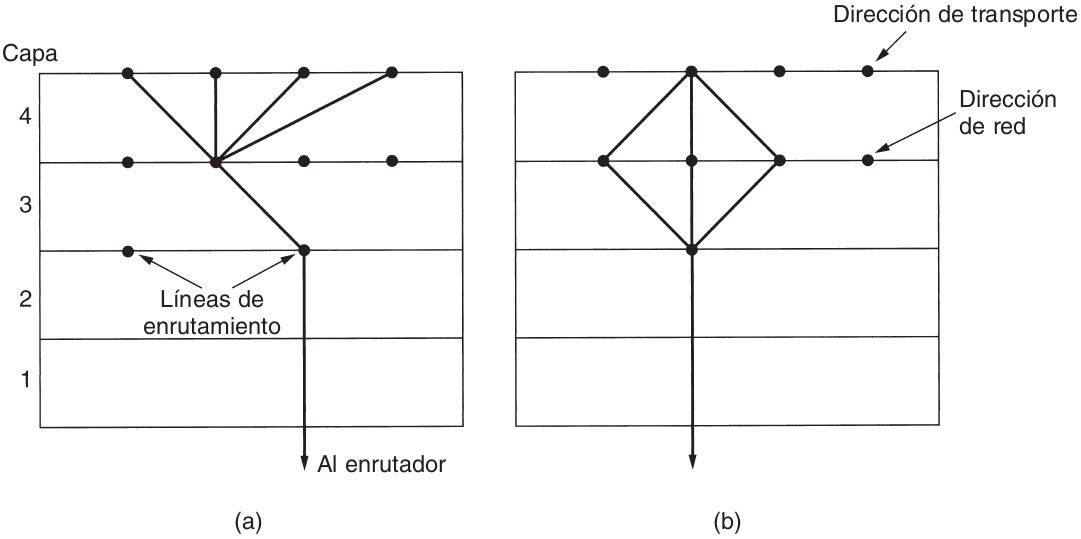
\includegraphics[width=0.8\textwidth-\fboxrule-\fboxrule]{imgs/multiplexion.png}}
\end{figure}

\subsection{Los Protocolos de Transporte de Internet: UDP}

Internet tiene dos protocolos principales en la CdT:
\begin{itemize}
\item \textbf{UDP (Protocolo de Datagrama de Usuario)}, no orientado a la conexión.
\item \textbf{TCP (Protocolo de Control de Transmisión)}, orientado a la conexión.
\end{itemize}

\subsubsection{Introducción a UDP}

Proporciona una forma para que las aplicaciones envíen datagramas IP encapsulados sin tener que establecer una conexión. Es un servicio sencillo, pero \textbf{no confiable}.

Se utiliza en los siguientes casos:
\begin{itemize}
\item El intercambio de mensajes es muy escaso. \textit{Ejemplo: consultas al DNS}.
\item La aplicación es en tiempo real. \textit{Ejemplo: Videoconferencias, VoIP}.
\item Los mensajes se envían regularmente y no importa si se pierde alguno. \textit{Ejemplo: SNMP}.
\item Se envía trafico \textit{broadcast}/\textit{multicast}.
\item Tráfico de P2P o IPTV.
\end{itemize}

UDP transmite \textbf{segmentos} que consisten en un encabezado de 8 \texttt{bytes} seguido por la carga útil. Agregamos los campos de \textbf{puertos de origen y destino} al formato IP puro. Con ellos, entrega los segmentos de manera correcta.

El \textbf{puerto de origen} se necesita principalmente cuando debe enviarse una respuesta al origen. Al copiar el campo \textit{Puerto de origen} del segmento que llega en el campo \textit{Puerto de destino} del segmento que sale, el proceso que envía la respuesta puede especificar cuál proceso de la máquina emisora va a obtenerlo.

\begin{figure}[ht!]
  \caption{Encabezado UDP.}
  \label{fig:udp}
  \centerline{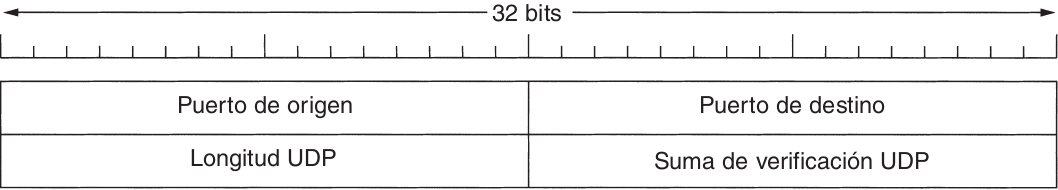
\includegraphics[width=0.85\textwidth-\fboxrule-\fboxrule]{imgs/udp.png}}
\end{figure}

El campo \textit{Longitud UDP} incluye el encabezado de 8 bytes y los datos. El campo \textit{Suma de verificación UDP} es opcional y se almacena como 0 si no se calcula (si la calidad del servicio no importa).

UDP proporciona una interfaz al protocolo IP con la característica agregada de desmultiplexar varios procesos utilizando los puertos, y efectúa opcionalmente una comprobación de errores. \textbf{No realiza}:

\begin{multicols}{2}
\begin{itemize}
\item Conexión/Desconexión.
\item Control de Flujo/Congestión.
\item Retransmisión de datos perdidos.
\end{itemize}
\end{multicols}

\subsection{Los Protocolos de Transporte de Internet: TCP}

La mayoría de las aplicaciones de Internet se necesita una entrega en secuencia \textbf{confiable}. UDP no puede proporcionar esto, en su lugar se utiliza TCP.

\subsubsection{Introducción a TCP}

Se diseño específicamente para proporcionar un flujo de \texttt{bytes} \textbf{confiable} de extremo a extremo a través de una interred \textbf{no confiable}. TCP tiene un diseño que se adapta de manera dinámica a las propiedades de la interred\footnote{Una \textbf{interred} difiere de una sola red debido a que diversas partes podrían tener diferentes topologías, anchos de banda, retardos, tamaños de paquete y otros parámetros.} y que se sobrepone a muchos tipos de fallas. Los paquetes TCP se llaman \textbf{segmentos}.

\textit{La capa IP no proporciona ninguna garantía de que los datagramas se entregarán de manera apropiada, por lo que corresponde a TCP proporcionar la confiabilidad que la mayoría de los usuarios desean y que IP no proporciona.}

\begin{wrapfigure}[21]{r}{0.35\textwidth}
  \caption{Algunos puertos asignados.}
  \label{fig:puertos}
  \centering
  \hbox{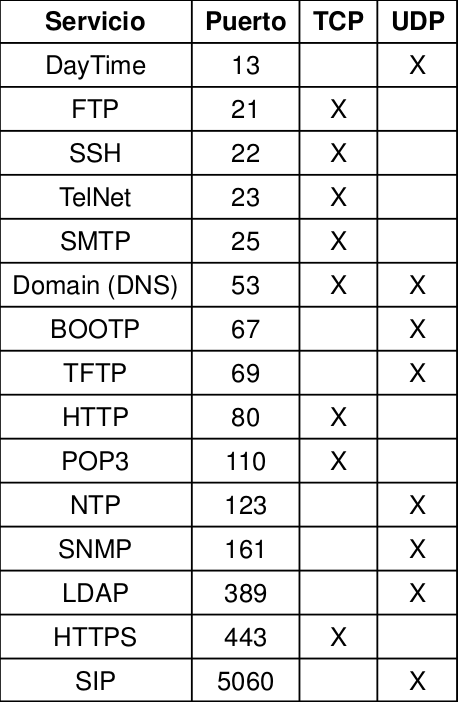
\includegraphics[width=0.35\textwidth-\fboxrule-\fboxrule]{imgs/puertos.png}}
\end{wrapfigure}

\subsubsection{El modelo del servicio TCP}

El servicio TCP se obtiene al hacer que tanto el servidor como el cliente creen puntos terminales, llamados \textbf{\textit{sockets}}. Cada \textit{socket} posee el número de dirección IP del \textit{host} y un número que es local a ese \textit{host}, llamado \textbf{puerto}. 

Los números de puerto menores que 1024 se llaman \textbf{puertos bien conocidos} y se reservan para servicios estándar. Para evitar que haya muchos \textit{daemons} de procesos inactivos la mayor parte del tiempo, se tiene un sólo \textit{daemon} llamado \textbf{inetd (Internet's daemon)} que se conecta a sí mismo a múltiples puertos y gestiona las conexiones de los \textit{daemons} de los otros procesos.

\textbf{Todas} las conexiones TCP son de \textbf{dúplex total} y de \textbf{punto a punto}. Algunas otras funciones que TCP lleva adelante son:

\begin{itemize}
\item Conexión/Desconexión.
\item Control de Congestión/Flujo.
\item Control de errores, retransmitiendo segmentos perdidos o erróneos. Elimina duplicados.
\item Gestión del intercambio de datos de forma eficiente en la red.
\end{itemize}

\subsubsection{El Protocolo TCP}

La entidad TCP emisora y la receptora intercambian datos en forma de segmentos. Un \textbf{segmento} consiste en un encabezado TCP fijo de \texttt{20 bytes} (más una parte opcional) seguido de cero o más \texttt{bytes} de datos. El \textit{software} de TCP decide el tamaño de los segmentos; puede acumular datos de varias escrituras para formar un segmento, o dividir los datos de una escritura en varios segmentos. Hay dos límites que restringen el tamaño de segmento:
\begin{enumerate} 
\item Cada segmento, incluido el encabezado TCP, debe caber en la carga útil de $\approx$\texttt{64Kb} del IP.
\item Cada red tiene una \textbf{unidad máxima de transferencia (MTU)} (generalmente de \texttt{1500 bytes}) y cada segmento debe caber en la MTU.
\end{enumerate}

El protocolo básico usado por las entidades TCP es el protocolo de \textbf{ventana corrediza}: Cuando llega un segmento al destino, la entidad TCP receptora devuelve un segmento que contiene un número de \texttt{ACK} igual al siguiente número de secuencia que espera recibir. Si el temporizador del emisor expira antes del \texttt{ACK} el emisor envía de nuevo el segmento.

\begin{figure}[ht!]
  \caption{Encabezado TCP.}
  \label{fig:encabezado_TCP}
  \centerline{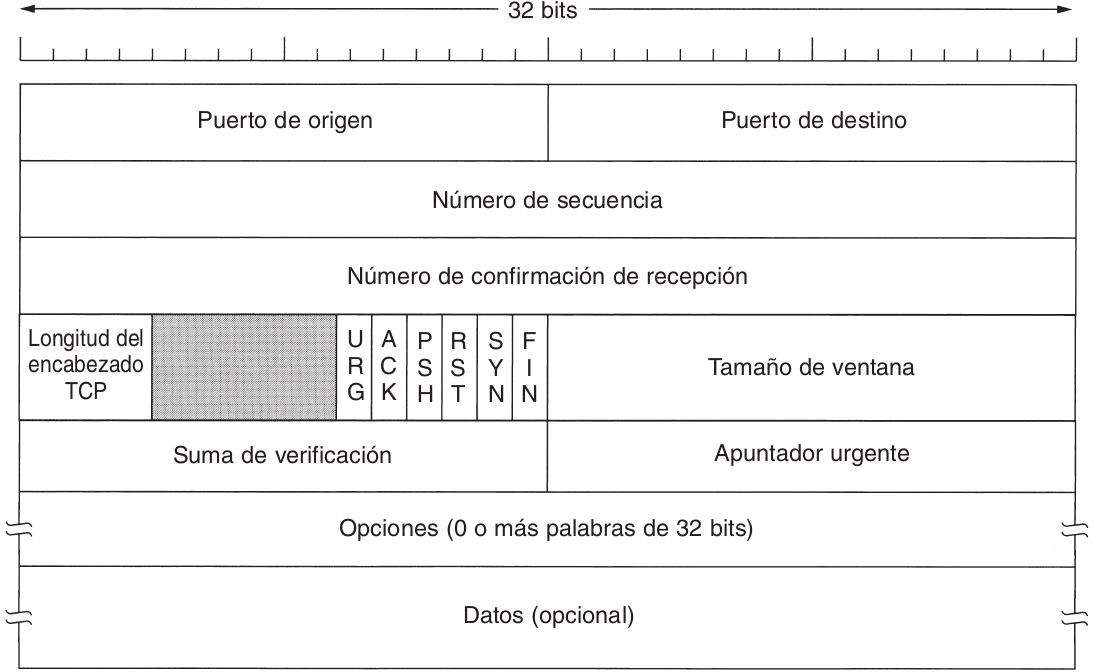
\includegraphics[width=0.9\textwidth-\fboxrule-\fboxrule]{imgs/encabezado_TCP.png}}
\end{figure}

\subsubsection{El encabezado del segmento TCP}

Contiene los siguientes campos:
\begin{multicols}{2}
\begin{itemize}
\item \textbf{Puerto origen y destino}. Identifican los puntos terminales locales de
la conexión.
\item \textbf{Numero de secuencia y de \texttt{ACK}}. El segundo especifica el siguiente \texttt{byte} esperado.
\item \textbf{Longitud del encabezado}. Indica la cantidad de palabras de \texttt{32 bits} contenidas en el encabezado TCP.
\item \textbf{URG}. Apuntador urgente. Interrumpe la aplicación receptora y le obliga a que lea los datos urgentes.
\item \textbf{ACK}. Se establece en 1 si la confirmación es válida.
\item \textbf{PSH}. Indica datos que se deben transmitir inmediato (no que queden almacenados).
\item \textbf{RST}. Restablece una conexión.
\item \textbf{SYN}. Para estabecer una conexión. Se usa para denotar \texttt{CR} y \texttt{CA}.
\item \textbf{FIN}. Para liberar una conexión.
\item \textbf{Tamaño de ventana}. Indica la cantidad de \texttt{bytes} que pueden enviarse comenzando por el \texttt{byte} cuya recepción se ha confirmado.
\item \textbf{Suma de verificación}. Agrega confiabilidad. Es una suma de verificación del
encabezado, los datos y el \textit{pseudoencabezado conceptual}.
\item \textbf{Opciones}. Ofrece una forma de agregar características extras no cubiertas por el encabezado normal. \textit{Ejemplo: Carga útil máxima que esta dispuesta a aceptar.}
\end{itemize}
\end{multicols}

\subsubsection{Establecimiento de una conexión TCP}

Se establecen usando el \textbf{acuerdo de tres vías}:
\begin{itemize}
\item El servidor espera pasivamente una conexión entrante ejecutando las primitivas \texttt{LISTEN} y \texttt{ACCEPT}, especificando o no el origen.
\item El cliente ejecuta una primitiva \texttt{CONNECT} especificando la dirección y el puerto IP. Esta primitiva envía un segmento TCP con el \texttt{bit SYN} encendido y el \texttt{bit ACK} apagado.
\item Si el servidor le rechaza, le envía un segmento con el \texttt{RST} encendido.
\item Si el servidor acepta, le envía un segmento de ACK.
\end{itemize}

\subsubsection{Liberación de una conexión TCP}

Para liberar una conexión, cualquiera de las partes puede enviar un segmento TCP con el \texttt{bit FIN} establecido, lo que significa que no tiene más datos por transmitir. Al confirmarse la recepción del \texttt{FIN}, ese sentido se apaga. Sin embargo, puede continuar un flujo de datos indefinido en el otro sentido. Cuando ambos sentidos se han apagado, se libera la conexión.

Se usan cuatro segmentos (o tres si hay \textit{piggybacking}). Se usan temporizadores para evitar el problema de los dos ejercitos.

\subsubsection{Política de transmisión del TCP}

Cuando la ventana es de 0, el emisor normalmente no puede enviar segmentos, salvo en dos situaciones:
\begin{enumerate}
\item Datos urgentes para enviar.
\item El emisor envia un segmento de \texttt{1 byte} para que el receptor reanuncie el siguiente \texttt{byte} esperado y el tamaño de la ventana.
\end{enumerate}

Para mejorar el desempeño del TCP, se debe lograr que el emisor no envíe segmentos pequeños, y que el receptor no los pida.

\subsubsection{Control de congestión en TCP}

El primer paso del manejo de la congestión es su detección. Para manejar la congestión TCP maneja dinámicamente el tamaño de las ventanas, asumiendo que existen dos problemas potenciales: \textbf{capacidad de la red} y \textbf{capacidad del receptor}.

Para solucionarlos, cada emisor mantiene dos ventanas:
\begin{itemize}
\item La ventana que ha otorgado el receptor.
\item La \textbf{ventana de congestión}.
\end{itemize}

La cantidad de \texttt{bytes} que pueden enviarse es la cifra menor de las dos ventanas.

\underline{\textbf{Algoritmo de arranque lento:}}

Al establecer una conexión, el emisor asigna a la ventana de congestión el \textbf{tamaño de segmento máximo} usado por la conexión; entonces envía un segmento máximo. Si se recibe la ACK de este segmento antes de que expire el temporizador, el emisor agrega el equivalente en \texttt{bytes} de un segmento a la ventana de congestión para hacerla de dos segmentos de tamaño máximo, y envía dos segmentos. A medida que se confirma cada uno de estos segmentos, se aumenta el tamaño de la ventana de congestión en un segmento máximo. La ventana de congestión sigue creciendo \textbf{exponencialmente} hasta ocurrir una expiración del temporizador o alcanzar el tamaño de la ventana receptora.

\begin{figure}[ht!]
  \caption{Ejemplo de algoritmo de arranque lento.}
  \label{fig:arranque_lento}
  \centerline{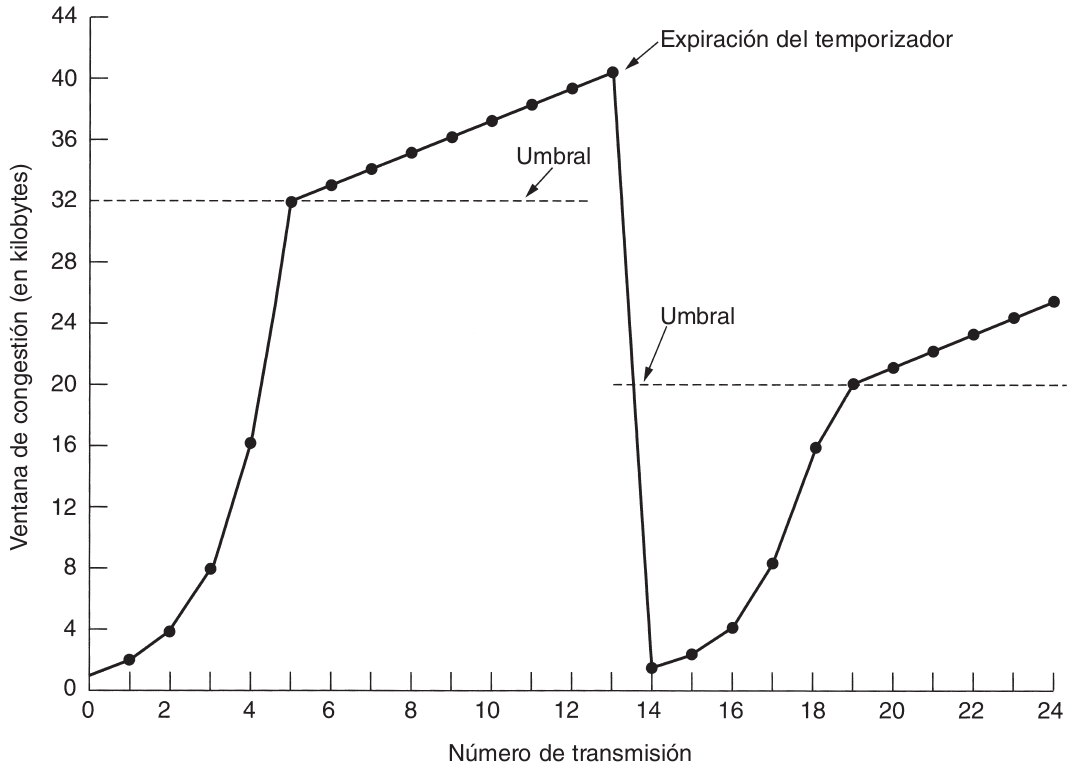
\includegraphics[width=0.85\textwidth-\fboxrule-\fboxrule]{imgs/arranque_lento.png}}
\end{figure}

Al ocurrir una expiración del temporizador, se establece el \textbf{umbral} en la mitad de la ventana de congestión actual, y la ventana de congestión se restablece a un segmento máximo. Luego se usa el \textit{arranque lento} para determinar lo que puede manejar la red, excepto que el crecimiento exponencial termina al alcanzar el umbral. A partir de este punto, las transmisiones exitosas aumentan linealmente la ventana de congestión (en un segmento máximo por ráfaga) en lugar de uno por segmento. En efecto, este algoritmo está suponiendo que probablemente es aceptable recortar la ventana de congestión a la mitad, y luego aumentarla gradualmente a partir de ahí.

\subsubsection{Administración de temporizadores del TCP}

El TCP usa conceptualmente varios temporizadores:
\begin{description}
\item \textbf{Temporizador de retransmisión.} Se inicia al enviarse un segmento. Si la ACK del segmento llega antes de expirar el temporizador, éste se detiene. Si, por otra parte, el temporizador termina antes de llegar la ACK, se retransmite el segmento. Este temporizador es ajustado constantemente con base de mediciones continuas del desempeño de la red.
\item \textbf{Temporizador de persistencia.} Es para evitar que el emisor y receptor se queden esperando en base a una falla de entrega de paquetes (\textbf{bloqueo irreversible}). Al expirar, el receptor envía un sondeo al receptor pidiéndole el estado del tamaño de su ventana.
\item \textbf{Temporizador de seguir con vida.} Cuando una conexión ha estado inactiva durante demasiado tiempo, el temporizador expira y comprueba el estado del otro lado: si no recibe respuesta, termina la conexión.
\item \textbf{Temporizador que usa \textit{Timed Wait}.} Se usa durante el cierre. Opera durante el doble del tiempo máximo de vida de paquete para asegurar que, al cerrarse una conexión, todos los paquetes creados por ella hayan desaparecido.
\end{description}

\end{document}